\chapter{Fault Tolerant Clustering}
\label{chap:tolerance}

Task clustering has been proven to be an effective method to reduce execution overhead and thereby the workflow makespan. However, a job composed of multiple tasks may have a greater risk of suffering from failures than a job composed of a single task. In this chapter, we demonstrate that transient failures can have a significant impact on the runtime performance of scientific workflows that use existing clustering policies that ignore failures. We optimize the workflow makespan by dynamically adjusting the clustering granularity in the presence of failures. We also propose a general task failure modeling framework and use a Maximum Likelihood Estimation based parameter estimation process to address these performance issues. We further propose three methods to improve the runtime performance of executing workflows in faulty environments. A trace based simulation is performed and it shows that our methods improve the workflow makespan significantly for five important applications.    

\section{Motivation}


In task clustering, a clustered job consists of multiple tasks. A task is marked as failed (task failure) if it is terminated by unexpected events during the computation of this task. If a task within a job fails, this job has a job failure, even though other tasks within this job do not necessarily fail. 
In a faulty environment, there are several options for reducing the influence of workflow failures. First, one can simply retry the entire job when its computation is not successful as in the Pegasus \cite{Deelman2004}, ASKALON \cite{fahringer2007askalon} and Chemomentum \cite{schuller2008chemomentum}. However, some of the tasks within the job may have completed successfully and it could be a waste of time and resources to retry all of the tasks. Second, the application process can be periodically checkpointed such that when a failure occurs, the amount of work to be retried is limited. However, the overheads of checkpointing can limit its benefits \cite{Zhang2004}. Third, tasks can be replicated to different nodes to avoid failures that are related to one specific worker node \cite{Plankensteiner2009}. However, inappropriate clustering (and replication) parameters may cause severe performance degradation if they create long-running clustered jobs. As we will show, a long-running job that consists of many tasks has a higher job failure rate even when the inter-arrival time of failures is long. 

We view the sequence of failure events as a stochastic process and study the distribution of its inter-arrival times, i.e. the time between failures. Our work is based on an assumption that the the distribution parameter of the inter-arrival time is a function of the \emph{type of task}. Tasks of the same type have the same computational program (executable file). In the five workflows we examine in this chapter, tasks at the same horizontal level (defined as the longest distance from the entry task of the workflow) of the workflows has the same type. 
The characteristics of tasks such as the task runtime, memory peak and disk usage are highly related to the task type \cite{da2013toward, Juve2013}.
Task type related failure is a type of failure that only occurs to some specific types of tasks. Samak \cite{Samak2011} et al. have analyzed 1,329 real workflow executions across six distinct applications and concluded that the type of a task is among the most significant factors that impacted failures. 

We propose two horizontal methods and one vertical methods to improve the existing clustering techniques in a faulty environment. The first horizontal method retries the failed tasks within a job. The second horizontal solution dynamically \emph{adjusts the granularity or clustering size} (number of tasks in a job) according to the estimated inter-arrival time of task failures. The vertical method reduces the clustering size by half in each job retry. 
%We further analyze the runtime performance of combining horizontal methods and vertical methods in different ways. 
We assume a task-level monitoring service is available. A task-level monitor tells which tasks in a clustered job fail or succeed, while a job-level monitor only tells whether this job fail or not. The job-level fault tolerant clustering has been discussed in our prior work \cite{Chen2012}. 



%A node failure only occurs to some specific execution nodes. 
Compared to our prior work in \cite{Chen2012}, we add a parameter learning process to estimate the distribution of the task runtime, the system overhead and the inter-arrival time of failures. We adopt an approach of prior and posterior knowledge based Maximum Likelihood Estimation (MLE) that has been recently used in machine learning. Prior knowledge about the parameters are modeled as a distribution with known parameters. Posterior knowledge about the execution information are also modeled a distribution with a known \emph{shape parameter} and an unknown \emph{scale parameter}. The shape parameter affects the shape of a distribution and the scale parameter affects the stretching or shrinking of a distribution. Both parameters control the characteristics of a distribution. The distribution of the prior and the posterior are in the same family if the likelihood distribution follows some specific distribution and they are called \emph{conjugate distributions}. For example, if the likelihood is a Weibull distribution and we model prior knowledge as an Inverse-Gamma distribution, then the posterior is also an Inverse-Gamma distribution. This simplifies the estimation of parameters and integrates the prior knowledge and posterior knowledge gracefully. More specifically, we define the parameter learning process with only prior knowledge as the static estimation. The process with both prior knowledge and posterior knowledge is called the dynamic estimation since we update the MLE based on the information collected during the execution.  

The two horizontal methods were introduced and evaluated in \cite{Chen2012} on two workflows. We complement this previous paper by studying (\emph{i}) the performance gain of using two horizontal methods and one vertical method over a baseline execution on a larger set of workflows (five widely used scientific applications); (\emph{ii}) the performance impact of the variance of the distribution of the task runtime, the system overheads and the inter-arrival time of failures; (\emph{iii}) the performance difference of dynamic estimation and static estimation with variation of inter-arrival time of failures.  


\section{Approach}


In this chapter, the \emph{goal} is to reduce the workflow makespan in a faulty environment by adjusting the clustering size ($k$). In task clustering, the clustering size ($k$) is an important parameter to influence the performance. We define it as the number of tasks in a clustered job. The reason why task clustering can help improve the performance is that it can reduce the scheduling cycles that workflow tasks go through since the number of jobs has decreased. The result is a reduction in the scheduling overhead and possibly other overheads as well \cite{Chen2011}. Additionally, in the ideal case without any failures, the clustering size is usually equal to the number of all the parallel tasks divided by the number of available resources. Such a naive setting assures that the number of jobs is equal to the number of resources and the workflow can utilize the resources as much as possible. However, when transient failures exist, we claim that the clustering size should be set based on the failure rates especially the task failure rate. Intuitively speaking, if the task failure rate is high, the clustered jobs may need to be re-executed more often compared to the case without clustering. Such performance degradation will counteract the benefits of reducing scheduling overheads. In the rest of this chapter, we will show how to adjust $k$ based on the estimated parameters of the task runtime $\bm t$, the system overhead $\bm s$ and the inter-arrival time of task failures $\bm\gamma$. 

\subsection{Task Failure Model}

%For system overhead $p(X|\theta)$, we assume it follows an Weibull distribution with known shape $\phi=0.78$. When $x>0$, the PDF of $p(x|\theta, \phi)$ is

%\begin{equation}
%f(x|\theta, \phi)=\frac{\phi}{\theta} (\frac{x}{\theta})^{\phi-1}e^{-(x/\theta)^{\phi}}  \nonumber
%\end{equation}


In our prior work \cite{Chen2011}, we have verified that system overheads $\bm s$ fits Gamma or Weibull distribution better than the other two distributions (Exponential and Normal). Schroeder et. al. \cite{Schroeder2006} have verified the inter-arrival time of task failures fits a Weibull distribution with a shape parameter of 0.78 better than lognormal and exponential distribution. We will reuse this shape parameter of 0.78 in our failure model. 
In \cite{Sun2003, Iosup2008} Weibull, Gamma and Lognormal distribution are among the best fit for the workflow traces they used.  Without loss of generality, we choose Gamma distribution to model the task runtime ($\bm t$) and the system overhead ($\bm s$) and use Weibull distribution to model the inter-arrival times of failures ($\bm\gamma$).  $\bm s$, $\bm t$ and $\bm \gamma$ are all random variables of all tasks instead of one specific task. 

Probability distributions such as Weibull and Gamma are usually described with two parameters: the \emph{shape parameter} ($\phi$) and the \emph{scale parameter} ($\theta$). The shape parameter affects the shape of a distribution and the scale parameter affects the stretching or shrinking of a distribution. Both of them control the characteristics of a distribution. For example, the mean of a Gamma distribution is $\phi\theta$ and the Maximum Likelihood Estimation or MLE is $(\phi-1)\theta$. 

Assume $a,b$ are the parameters of the prior knowledge, $D$ is the observed dataset and $\theta$ is the parameter we aim to estimate. In Bayesian probability theory, if the posterior distribution $p(\theta|D, a, b)$ are in the same family as the prior distribution $p(\theta|a, b)$, the prior and the posterior are then called conjugate distributions, and the prior is called a conjugate prior for the likelihood function. For example, the Inverse-Gamma family is conjugate to itself (or self-conjugate) with respect to a Weibull likelihood function: if the likelihood function is Weibull, choosing an Inverse-Gamma prior over the mean will ensure that the posterior distribution is also Inverse-Gamma. This simplifies the estimation of parameters since we can reuse the prior work from other researchers \cite{Schroeder2006, Iosup2008, Sun2003, Chen2011} on the failure analysis and performance analysis. 

After we observe data $D$, we compute the posterior distribution of $\theta$:

\begin{eqnarray*}
	\displaystyle  
	p(\theta|D, a, b)&=&\frac{p(\theta|a, b)\times p(D|\theta)}{p(D|a, b)}\nonumber  \\
	&\propto&p(\theta|a, b)\times p(D|\theta)\nonumber 
\end{eqnarray*}

$D$ can be the observed inter-arrival time of failures $X$, the observed task runtime $RT$ or the observed system overheads $S$. 
$X=\{x_1, x_2, ..., x_n\}$ is the observed data of $\bm\gamma$ during the runtime. Similarly, we define $RT=\{t_1, t_2, ..., t_n\}$ and $S=\{s_1, s_2, ..., s_n\}$ as the observed data of $\bm t$ and $\bm s$ respectively. $p(\theta|D,a, b)$ is the posterior that we aim to compute. $p(\theta|a, b)$ is the prior, which we have already known from previous work. $p(D|\theta)$ is the likelihood. 
%We only need to know its shape parameter instead of its scale parameter, which reduces the work to estimate its scale parameter. 



More specifically, we model the inter-arrival time of failures ($\bm\gamma$) with a Weibull distribution as \cite{Schroeder2006} that has a known shape parameter of $\phi_{\gamma}$ and an unknown scale parameter $\theta_{\gamma}$: $\bm\gamma\sim W(\theta_{\gamma}, \phi_{\gamma})$. 

The conjugate pair of a Weibull distribution with a known shape parameter $\phi_{\gamma}$ is an Inverse-Gamma distribution, which means if the prior follows an Inverse-Gamma distribution $\Gamma^{-1}(a_{\gamma}, b_{\gamma})$ with the shape parameter as $a_{\gamma}$ and the scale parameter as $b_{\gamma}$, then the posterior follows an Inverse-Gamma distribution:

\begin{equation}
\label{eq:theta_1}
\theta_{\gamma}\sim\Gamma^{-1}(a_{\gamma}+n,\displaystyle b_{\gamma}+\sum_{i=1}^n{x_i^{\phi_{\gamma}}})
 \end{equation}

The MLE (Maximum Likelihood Estimation) of the scale parameter $\theta_{\gamma}$ is:

\begin{equation}
MLE(\theta_{\gamma})=\displaystyle\frac{b_{\gamma}+\displaystyle\sum_{i=1}^n{x_i^{\phi_{\gamma}}}}{a_{\gamma}+n+1}
\end{equation}

The understanding of the MLE has two folds: initially we do not have any data and thus the MLE is $\displaystyle\frac{b_{\gamma}}{a_{\gamma}+1}$, which means it is determined by the prior knowledge; when $n\to\infty$, the MLE $\displaystyle\frac{\displaystyle\sum_{i=1}^n{x_i^{\phi_{\gamma}}}}{n+1}\to\overline{x^{\phi_{\gamma}}}$, which means it is determined by the observed data and it is close to the regularized average of the observed data. The static estimation process only utilizes the prior knowledge and the dynamic estimation process uses both the prior and the posterior knowledge. 

We model the task runtime ($\bm t$) with a Gamma distribution as \cite{Sun2003, Iosup2008} with a known shape parameter $\phi_{t}$ and an unknown scale parameter $\theta_t$. The conjugate pair of Gamma distribution with a known shape parameter is also a Gamma distribution. If the prior follows $\Gamma(a_t, b_t)$, while $a_t$ is the shape parameter and $b_t$ is the rate parameter (or $\displaystyle \frac{1}{b_t}$ is the scale parameter), the posterior follows $\Gamma(a_t+n\phi_t, b_t+\displaystyle\sum_{i=1}^n{t_i})$ with $a_t+n\phi_t$ as the shape parameter and $b_t+\displaystyle\sum_{i=1}^n{t_i}$ as the rate parameter. The MLE of $\theta_t$ is $\displaystyle\frac{b_t+\displaystyle\sum_{i=1}^n{t_i}}{a_t+n\phi_t-1}$. 

Similarly, if we model the system overhead $\bm s$ with a Gamma distribution with a known shape parameter $\phi_{s}$ and an unknown scale parameter $\theta_s$, and the prior is $\Gamma(a_s, b_s)$, the MLE of $\theta_s$ is $\displaystyle\frac{b_s+\displaystyle\sum_{i=1}^n{s_i}}{a_s+n\phi_s-1}$.
%Should not consider the resource

We have already assumed the task runtime, system overhead and inter-arrival time between failures are a function of task types. Since in scientific workflows, tasks at the different level (the deepest depth from the entry task to this task) are usually of different type, we model the runtime level by level. Given $n$ independent tasks at the same level and the distribution of the task runtime, the system overhead, and the inter-arrival time of failures, we aim to reduce the cumulative runtime $\bm M$ of completing these tasks by adjusting the clustering size $k$ (the number of tasks in a job). 
$\bm M$ is also a random variable and it includes the system overheads and the runtime of the clustered job and its subsequent retry jobs if the first try fails. We also assume the task failures are independent in each worker node (but with the same distribution) without considering the failures that brings the whole system down such as a failure in the shared file system. 
%since that is not the concern of task clustering but the task scheduling. 

The runtime of a job is a random variable indicated by $\bm d$. A clustered job succeeds only if all of its tasks succeed. The job runtime is the sum of the cumulative task runtime of $k$ tasks and a system overhead. We assume the task runtime of each task is independent of each other, therefore the cumulative task runtime of $k$ tasks is also a Gamma distribution since the sum of Gamma distributions with the same shape parameter is still a Gamma distribution. We also assume the system overhead is independent of all the task runtimes and it has the same shape parameter ($\phi_{ts}=\phi_{t}=\phi_{s}$) with the task runtime. 
%Don't know how to explain
%In practice, this assumption means the cumulative task runtime and the system overhead are generated at the same rate (or scale). 
%which is consistent with our o-DAG model that has one system overhead associated to one job. 
The job runtime irrespective of whether it succeeds of fails is:
\begin{eqnarray}
\displaystyle
\bm{d}\sim\Gamma(\phi_{ts}, k\theta_t+\theta_s)\\
MLE(\bm{d})=\displaystyle{(k\theta_t+\theta_s) }{(\phi_{ts}-1)}
\label{eq:N}
\end{eqnarray}
%We assume that $n \gg r$, but $n/k$ is not necessarily much larger than $r$ since $k$ could be very large. Normally at the beginning of workflow execution, $n/k > r$, which means there are more clustered jobs than available resources. To try all $n$ tasks once, irrespective of whether they succeed or fail, one needs approximately $\displaystyle \frac{n}{rk}$ execution cycle(s) since at each execution cycle we can execute at most $r$ jobs. Therefore, 

%We have assumed the task runtime $t\sim\Gamma^{-1}(a_t, b_t)$. $(a_t, b_t)$ are estimated from prior knowledge and/or posterior knowledge. The system overhead $s\sim\Gamma^{-1}(a_s, b_s)$ similarly. By merging the $k$ tasks together, their computational runtime still follows a Inverse-Gamma distribution with parameter $(a_t, kb_t)$. We use $\mathcal{L}(f)$ to indicate the Laplace transform of the distribution $f$ (time-series signal in Laplace transform). $d$ is a random variable that represents the job runtime, which includes the computational runtime of $k$ tasks and the system overhead $s$. The PDF of $d$ is: $M$ is a random variable represents the cumulative job runtime of $\displaystyle\frac{n}{k}$ jobs. For a given $M$, we have:

Let the retry time of clustered jobs to be $N$. The process to run and retry a job is a Bernoulli trial with only two results: success or failure. Once a job fails, it will be re-executed until it is eventually completed successfully since we assume the failures are transient. For a given job runtime $d_i$, by definition:
\begin{eqnarray}
\displaystyle
N_i=\frac{1}{1-F(d_i)}=\frac{1}{e^{-(\displaystyle\frac{d_i}{\theta_{\gamma}})^{\phi_{\gamma}}}}=e^{(\displaystyle\frac{d_i}{\theta_{\gamma}})^{\phi_{\gamma}}} 
\label{eq:N_i}
\end{eqnarray}

$F(x)$ is the CDF (Cumulative Distribution Function) of $\bm\gamma$. The time to complete $d_i$ successfully in a faulty environment is

\begin{eqnarray}
\displaystyle
M_i=d_iN_i=d_ie^{(\displaystyle\frac{d_i}{\theta_{\gamma}})^{\phi_{\gamma}}} 
\label{eq:M}
\end{eqnarray}

Equation \ref{eq:M} has involved two distributions $\bm d$ and $\theta_{\gamma}$ ($\phi_{\gamma}$ is known). From Equation \ref{eq:theta_1}, we have:

\begin{eqnarray}
\displaystyle\cfrac{1}{\theta_{\gamma}}\sim\Gamma(a_{\gamma}+n,\frac{1}{\displaystyle b_{\gamma}+\sum_{i=1}^n{x_i^{\phi_{\gamma}}}}) \\
MLE(\displaystyle\cfrac{1}{\theta_{\gamma}})=\displaystyle\cfrac{a_{\gamma}+n-1}{\displaystyle b_{\gamma}+\sum_{i=1}^n{x_i^{\phi_{\gamma}}}}
 \end{eqnarray}

$M_i$ is a monotonic increasing function of both $d_i$ and $\displaystyle\cfrac{1}{\theta_{\gamma}}$, and the two random variables are independent of each other, therefore:


\begin{equation} 
\label{eq:MLE-M-i}
MLE(M_i)=MLE(d_i)e^{(\displaystyle MLE(d_i)MLE(\cfrac{1}{\theta_{\gamma}}))^{\phi_{\gamma}}} 
\end{equation}

Equation \ref{eq:MLE-M-i} means to attain $MLE(M_i)$, we just need to attain $MLE(d_i)$ and $MLE(\cfrac{1}{\theta_{\gamma}})$ at the same time. 
In both dimensions ($d_i$ and $\displaystyle\cfrac{1}{\theta_{\gamma}}$), $M_i$ is a Gamma distribution and each $M_i$ has the same distribution parameters, therefore:

\begin{eqnarray} 
\label{eq:MLE-M}
\bm{M}&=&\displaystyle\cfrac{1}{r}\sum_{i=1}^{\cfrac{n}{k}}M_i\sim\Gamma \nonumber\\
MLE(\bm{M})&=&\displaystyle\cfrac{n}{rk}MLE(M_i)\\
&=&\displaystyle\cfrac{n}{rk} MLE(d_i)e^{(\displaystyle MLE(d_i)MLE(\cfrac{1}{\theta_{\gamma}}))^{\phi_{\gamma}}} 
\end{eqnarray}

$r$ is the number of resources. In this chapter, we consider a compute cluster as a homogeneous cluster, which is usually true in dedicated clusters and Clouds. 

%On the other side, at the end of the workflow execution, since n is decreasing with the process of workflow, it is possible that $\displaystyle \frac{n}{k} < r$, which means there are fewer jobs than the available resources. One needs just one execution cycle to execute these tasks once. The time to complete all $n$ tasks successfully is $N(kt+s)$. 

%In summary, the estimated overall runtime is, 

%\begin{equation} 
%\label{eq:jfm}
%M=
%\begin{cases}
%\cfrac{n(kt+s)}{rk}{e^{(\cfrac{kt+s}{\theta})^{\phi}}}, & \text{if } \cfrac{n}{k}\geq r \\
%(kt+s){e^{(\cfrac{kt+s}{\theta})^{\phi}}}, & \text{else}
%\end{cases}
%\end{equation}

Let $k^*$ be the optimal clustering size that minimizes Equation \ref{eq:MLE-M}.  $\arg min$  stands for the argument ($k$) of the minimum\footnote{Wiki: http://en.wikipedia.org/wiki/Arg\_max}, that is to say, the $k$ such that $MLE(\bm{M})$ attains its minimum value. 

\begin{eqnarray} 
\label{eq:k_optimal}
k^*=\arg min\{MLE(\bm{M})\} 
\end{eqnarray}

It is difficult to find a analytical solution of $k^*$. However, there are a few constraints that can simplify the estimation of $k^*$: (\emph{i}) $k$ can only be an integer in practice; (\emph{ii}) $MLE(\bm{M})$ is continuous and has one minimal. Methods such as Newton's method can be used to find the minimal $MLE(\bm{M})$ and the corresponding $k$. Figure~\ref{fig:model_makespan} shows an example of $MLE(\bm{M})$ using static estimation with a low task failure rate ($\theta_{\gamma}=40$s), a medium task failure rate ($\theta_{\gamma}=30$s) and a high task failure rate ($\theta_{\gamma}=20$s). Other parameters are $n=50$, $\theta_{t}=5$ sec, and $\theta_{s}=50$ sec and all the shape parameters are 2 for simplicity. These parameters are close to the level of mProjectPP in the Montage workflow that we simulate in Section \ref{sec:tolerance:experiments}. 
Figure \ref{fig:model_size} shows the relationship between the optimal clustering size ($k^*$) and $\theta_{\gamma}$, which is a non-decreasing function. The optimal clustering size (marked with red dots in Figure~\ref{fig:model_size}) when $\theta_{\gamma}=20,30,40$ is 4,5 and 6 respectively. 
 It is consistent with our expectation since the longer the inter-arrival time of failures is, the lower the task failure rate is. With a lower task failure rate, a larger $k$ assures that we reduce system overheads without retrying many times.  



\begin{figure*}[!htb]
\centering
  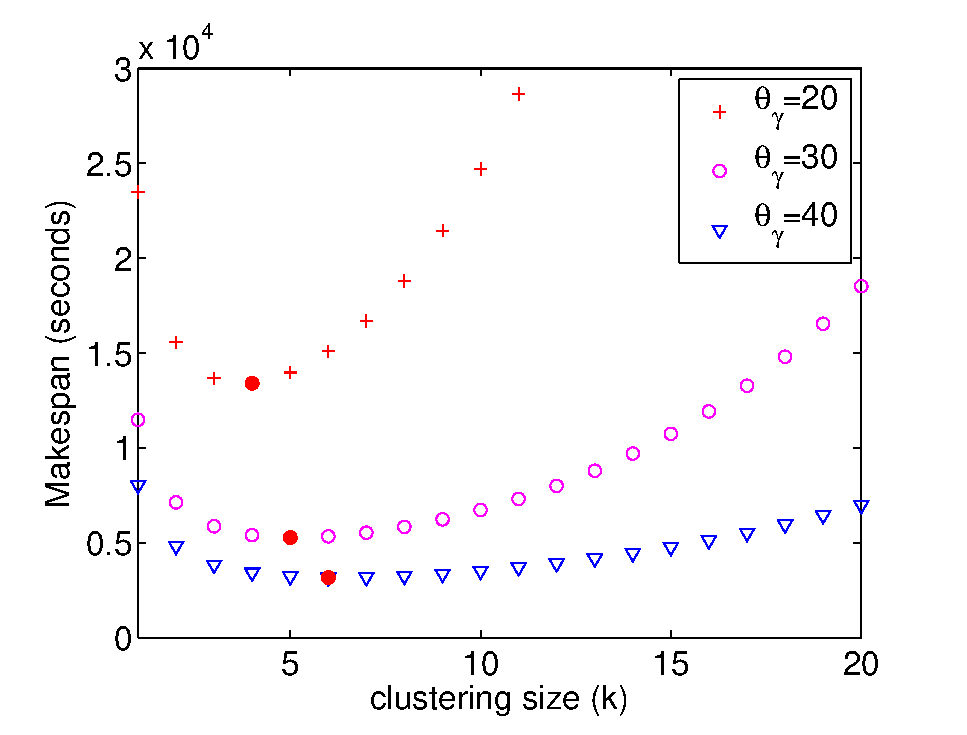
\includegraphics[width=0.55\linewidth]{figures/tolerance/model_makespan.eps}
  \caption{Makespan with different clustering size and $\theta_{\gamma}$. ($n=1000$, $r=20$, $\theta_t=5$ sec, $\theta_s=50$ sec). The red dots are the minimums. }
  \label{fig:model_makespan}
\end{figure*}

\begin{figure*}[!htb]
\centering
  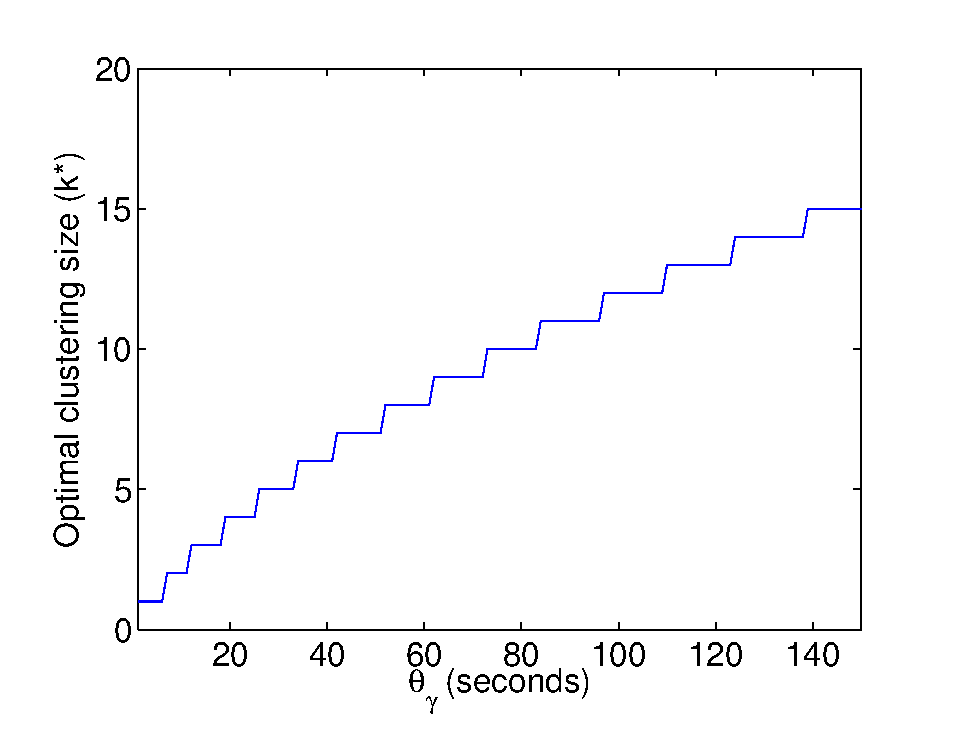
\includegraphics[width=0.55\linewidth]{figures/tolerance/model_size.eps}
  \caption{Optimal clustering size (k*) with different  $\theta_{\gamma}$ ($n=1000$, $r=20$, $\theta_t=5$ sec, $\theta_s=50$ sec)}
  \label{fig:model_size}
\end{figure*}


From this theoretic analysis, we conclude that (\emph{i}) the longer the inter-arrival time of failures is, the better runtime performance the task clustering has; (\emph{ii}), adjusting the clustering size according to the detected inter-arrival time can improve the runtime performance. 


\subsection{Fault Tolerant Clustering Methods}

To improve the fault tolerance from the point of view of clustering, we propose three methods: Dynamic Reclustering (\emph{DR}), Selective Reclustering (\emph{SR}) and Vertical Reclustering (\emph{VR}). In the experiments, we compare the performance of our fault tolerant clustering methods to an existing version of Horizontal Clustering (HC)~\cite{Singh2008} technique. In this subsection, we first briefly describe these algorithms.

\textbf{Horizontal Clustering} (\emph{HC}). 
Horizontal Clustering (HC) merges multiple tasks that are at the same horizontal level of the workflow. The clustering granularity (number of tasks within a cluster) of a clustered job is controlled by the user, who defines either the number of tasks per clustered job (\emph{clusters.size}), or the number of clustered jobs per horizontal level of the workflow (\emph{clusters.num}). This algorithm has been implemented and used in Pegasus~\cite{Singh2008}. For simplicity, we set \emph{clusters.num} to be the same as the number of available resources. In our prior work~\cite{Chen2013a,Chen2013b}, we have compared the runtime performance with different clustering granularity. The pseudocode of the HC technique is shown in Algorithm~\ref{alg:evaluation_hc}. The Clustering and Merge Procedure are called in the initial task clustering process while the Reclustering Procedure is called when there is a failed job returned. 

\begin{algorithm}[!htb]
	\footnotesize
	\caption{Horizontal Clustering algorithm.}
	\label{alg:evaluation_hc}
	\begin{algorithmic}[1]
		\Require $W$: workflow; $C$: max number of tasks per job defined by \emph{clusters.size} or \emph{clusters.num}
		\Procedure{Clustering}{$W,C$}
			\For{$level < depth(W)$}
				\State $TL\gets $\ \Call{GetTasksAtLevel}{$W,level$} \Comment{Partition $W$ based on depth}
				\State $CL\gets$  \ \Call{Merge}{$TL,C$} \Comment{Returns a list of clustered jobs}
				\State $W \gets W - TL + CL$  \Comment{Merge dependencies as well} 
			\EndFor
		\EndProcedure
		\Procedure{Merge}{$TL, C$}
			\State $J\gets$ \{\}\Comment{An empty job}
			\State $CL\gets$\{\}\Comment{An empty list of clustered jobs}
			\While{$TL$ is not empty}
				\State $J$.add ($TL$.pop($C$) \Comment{Pops $C$ tasks that are not merged }
				\State  $CL$.add( $J$)
			\EndWhile
			\State \textbf{return} $CL$
		\EndProcedure
		\Procedure{Reclustering}{$J$}\Comment{$J$ is a failed job}
			\State $J_{new}\gets$\ \Call{CopyOf}{$J$} \Comment{Copy Job $J$}
			\State $W \gets W + J_{new}$ \Comment{Re-execute it}
		\EndProcedure
	\end{algorithmic}
\end{algorithm}


\begin{figure*}[!htb]
\centering
  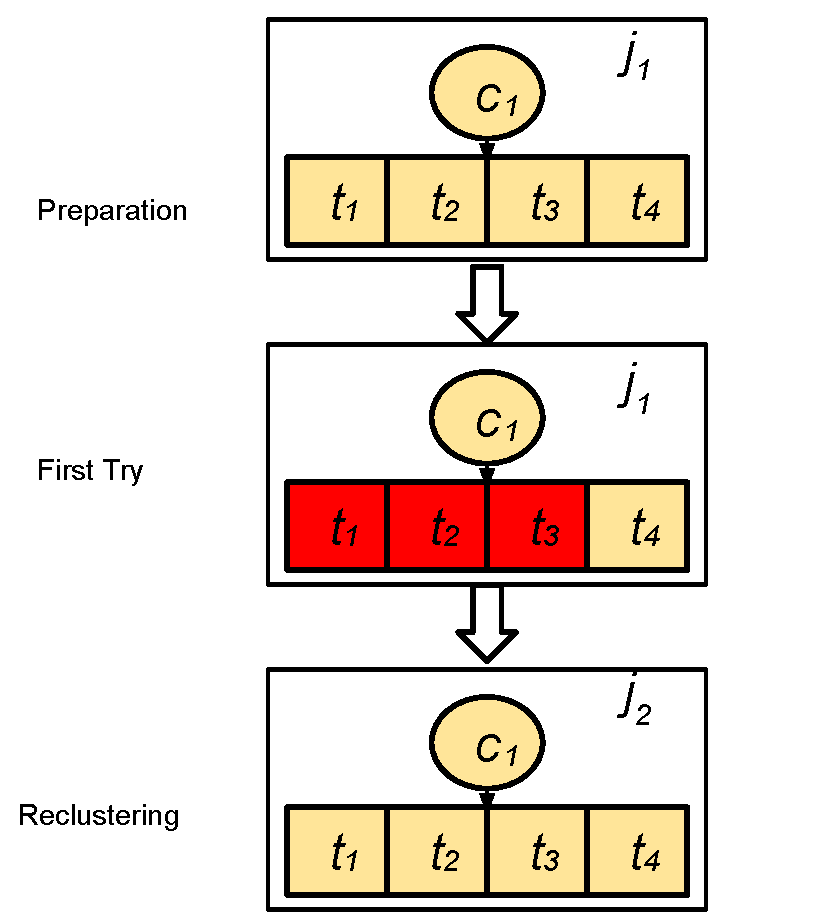
\includegraphics[width=0.4\linewidth]{figures/tolerance/hcr.pdf}
  \caption{Horizontal Clustering (red boxes are failed tasks)}
  \label{fig:clustering_hc}
\end{figure*}

%The type of tasks is used to detect the task specific failures and the resource id is used to detect location specific failures. 
Figure \ref{fig:clustering_hc} shows an example where the initial clustering size is 4 and thereby there are four tasks in a clustered job at the beginning. During execution, three out of these tasks ($t_1, t_2, t_3$) fail. HC will keep retrying all of the four tasks in next try until all of them succeed. Such a retry mechanism has been implemented and used in Pegasus~\cite{Singh2008}.




\begin{figure*}[!htb]
\centering
  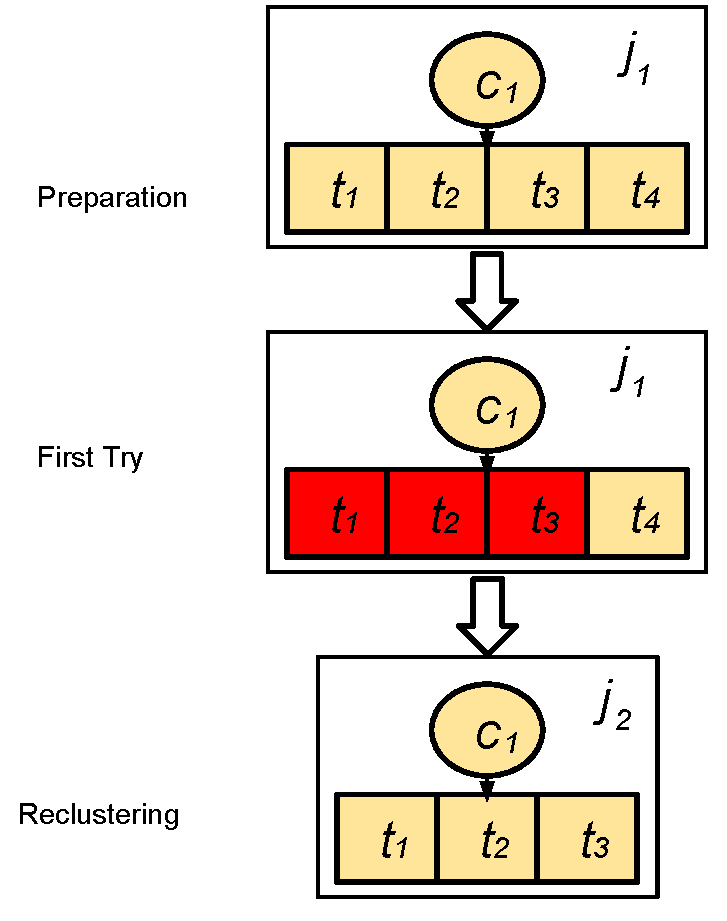
\includegraphics[width=0.35\linewidth]{figures/tolerance/sr.pdf}
  \caption{Selective Reclustering (red boxes are failed tasks)}
  \label{fig:clustering_sr}
\end{figure*}

\textbf{Selective Reclustering} (\emph{SR}). HC does not adjust the clustering size even when it continuously sees many failures. We further improve the performance with Selective Reclustering that selects the failed tasks in a clustered job and merges them into a new clustered job. SR is different to HC in that HC retries all tasks of a failed job even though some of the tasks have succeeded. 
%SR requires task level monitoring in workflow management systems. 

Figure \ref{fig:clustering_sr} shows an example of SR. At the first try, there are four tasks and three of them ($t_1, t_2, t_3$) have failed. One task ($t_4$) succeeds and exits. Only the three failed tasks are merged again into a new clustered job $j_2$ and the job is retried. This approach does not intend to adjust the clustering size, although the clustering size will be smaller and smaller spontaneously after each retry since there are less and less tasks in a clustered job. In this case, the clustering size has decreased from 4 to 3. However, the optimal clustering size may not be 3, which limits its performance if the $\theta_{\gamma}$ is small and $k$ should be decreased as much as possible. The advantage of SR is that it is simple to implement and be incorporated into existing workflow management systems without loss of much efficiency as shown in Section~\ref{sec:tolerance:experiments}. It also serves as a comparison with the Dynamic Reclustering approach that we propose below. Algorithm \ref{alg:evaluation_sr} shows the pseudocode of SR. The Clustering and Merge procedures are the same as those in HC. 

\begin{algorithm}[!htb]
	\footnotesize
	\caption{Selective Reclustering algorithm. }
	\label{alg:evaluation_sr}
	\begin{algorithmic}[1]
		\Require $W$: workflow; $C$: max number of tasks per job defined by \emph{clusters.size} or \emph{clusters.num}
			\Procedure{Reclustering}{$J$}\Comment{$J$ is a failed job}
			\State $TL \gets$\ \Call{GetTasks}{$J$}
			\State $J_{new}\gets$\{\}\Comment{An empty job}
			\ForAll{Task $t$ in $TL$}
				\If{$t$ is failed}
					\State $J_{new}$.add ($t$)
				\EndIf
			\EndFor
			\State $W \gets W + J_{new}$ \Comment{Re-execute it}
		\EndProcedure
	\end{algorithmic}
\end{algorithm}

 

\begin{figure*}[!htb]
\centering
  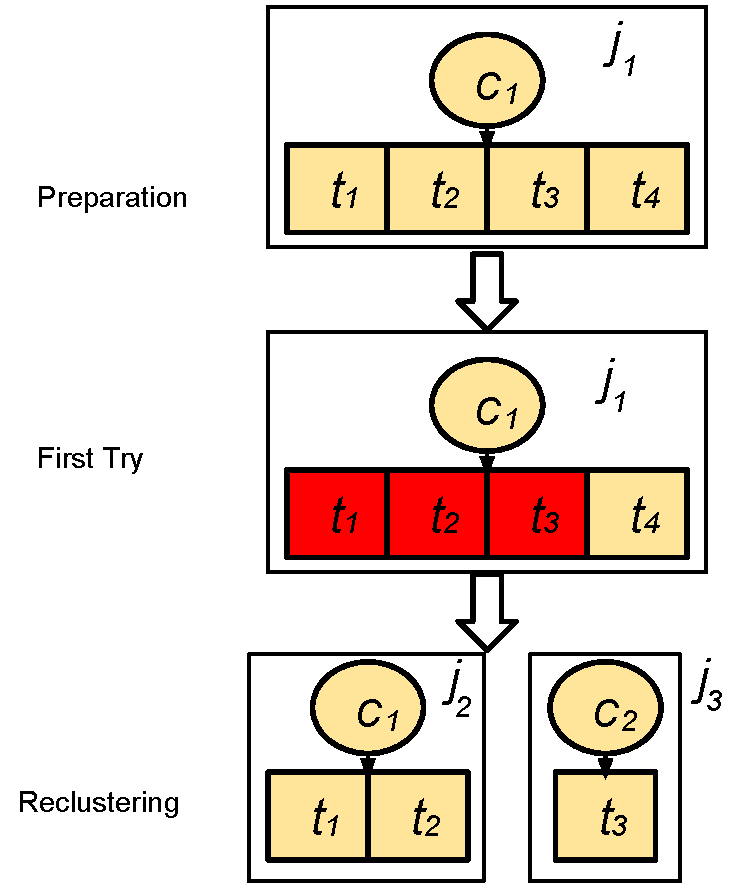
\includegraphics[width=0.4\linewidth]{figures/tolerance/dr.pdf}
  \caption{Dynamic Reclustering (red boxes are failed tasks)}
  \label{fig:clustering_dr}
\end{figure*}

\textbf{Dynamic Reclustering} (\emph{DR}). 
Selective Reclustering does not analyze the clustering size rather, it uses a self-adjusted approach to reduce the clustering size if the failure rate is too high. However, it is blind about the optimal clustering size and the actual clustering size may be larger or smaller than the optimal clustering size. We then propose the second method, Dynamic Reclustering. In DR, only failed tasks are merged into new clustered jobs and the clustering size is set to be $k^*$ according to Equation \ref{eq:k_optimal}.
% DR requires the ability to detect which tasks have failed in a job. 



Figure \ref{fig:clustering_dr} shows an example where the initial clustering size is 4 and thereby there are four tasks in a clustered job at the beginning. At the first try, three tasks within a clustered job have failed. Therefore we have only three tasks to retry and further we need to decrease the clustering size (in this case it is 2) accordingly. We end up with two new jobs $j_2$ (that has $t_1$ and $t_2$) and $j_3$ that has $t_3$. Algorithm \ref{alg:evaluation_dr} shows the pseudocode of DR. The Clustering and Merge procedures are the same as those in HC. 

\begin{algorithm}[!htb]
	\footnotesize
	\caption{Dynamic Reclustering algorithm.}
	\label{alg:evaluation_dr}
	\begin{algorithmic}[1]
		\Require $W$: workflow; $C$: max number of tasks per job defined by \emph{clusters.size} or \emph{clusters.num}
			\Procedure{Reclustering}{$J$}\Comment{$J$ is a failed job}
			\State $TL \gets$\ \Call{GetTasks}{$J$}
			\State $J_{new}\gets$\{\}
			\ForAll{Task $t$ in $TL$}
				\If{$t$ is failed}
					\State $J_{new}$.add ($t$)
				\EndIf
				\If{$J_{new}.size() > k^*$}
					\State $W \gets W + J_{new}$
					\State $J_{new}\gets$\{\}
				\EndIf
			\EndFor
			\State $W \gets W + J_{new}$ \Comment{Re-execute it}
		\EndProcedure
	\end{algorithmic}
\end{algorithm}

\begin{figure*}[!htb]
\centering
  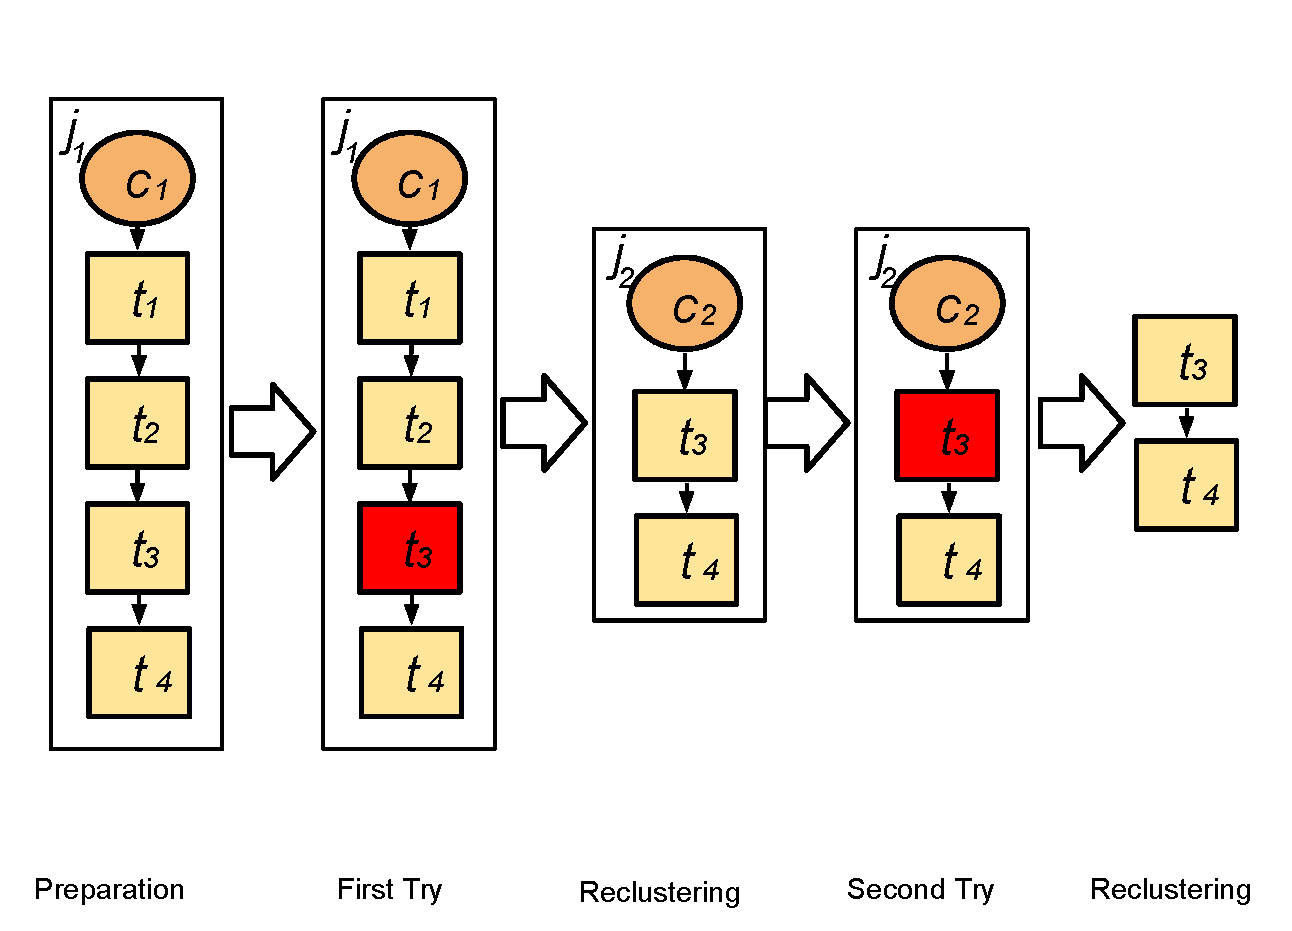
\includegraphics[width=0.65\linewidth]{figures/tolerance/vr.pdf}
  \caption{Vertical Reclustering (red boxes are failed tasks)}
  \label{fig:clustering_vr}
\end{figure*}

\textbf{Vertical Reclustering} (\emph{VR}). VR is an extension of Vertical Clustering. Similar to Selective Reclustering, Vertical Reclustering only retries tasks that are failed or not completed.
If there is a failure detected, we decrease $k$ by half and recluster them. In Figure \ref{fig:clustering_vr}, if there is no assumption of failures initially, we put all the tasks ($t_1, t_2, t_3, t_4$) from the same  pipeline into a clustered job. $t_3$ fails at the first try assuming it is a failure-prone task (its $\theta_{\gamma}$ is short). VR retries only the failed tasks ($t_3$) and tasks that are not completed ($t_4$) and merges them again into a new job $j_2$. In the second try, $j_2$ unfortunately fails and we divide it into two tasks ($t_3$ and $t_4$). Since the clustering size is already 1, VR performs no vertical clustering anymore and would continue retrying $t_3$ and $t_4$ (but still following their data dependency) until they succeed. Algorithm \ref{alg:evaluation_vr} shows the pseudocode of VR. 

\begin{algorithm}[!htb]
	\footnotesize
	\caption{Vertical Reclustering algorithm.}
	\label{alg:evaluation_vr}
	\begin{algorithmic}[1]
		\Require $W$: workflow; 
		\Procedure{Clustering}{$W$}
			\For{$level < depth(W)$}
				\State $TL\gets $\ \Call{GetTasksAtLevel}{$W,level$} \Comment{Partition $W$ based on depth}
				\State $CL, TL_{merged}\gets$  \ \Call{Merge}{$TL$} \Comment{Returns a list of clustered jobs}
				\State $W \gets W - TL_{merged} + CL$  \Comment{Merge dependencies as well} 
			\EndFor
		\EndProcedure
		\Procedure{Merge}{$TL$}
			\State $TL_{merged}\gets TL$\Comment{All the tasks that have been merged}
			\State $CL\gets$\{\}\Comment{An empty list of clustered jobs}
			\ForAll{$t$ in $TL$}
				\State $J\gets$ \{$t$\}
				\While{$t$ has only one child $t_{child}$ and $t_{child}$ has only one parent}
					\State $J$.add ($t_{child}$)
					\State $TL_{merged}\gets TL_{merged} + t_{child}$ 
					\State $t\gets t_{child}$
				\EndWhile
				\State  $CL$.add( $J$)
			\EndFor
			\State \textbf{return} $CL$, $TL_{merged}$
		\EndProcedure
		\Procedure{Reclustering}{$J$}\Comment{$J$ is a failed job}
			\State $TL \gets$\ \Call{GetTasks}{$J$}
			\State $k^*\gets J.size() / 2$ \Comment{Reduce the clustering size by half}
			\State $J_{new}\gets$\{\}
			\ForAll{Task $t$ in $TL$}
				\If{$t$ is failed or not completed}
					\State $J_{new}$.add ($t$)
				\EndIf
				\If{$J_{new}.size() > k^*$}
					\State $W \gets W + J_{new}$
					\State $J_{new}\gets$\{\}
				\EndIf
			\EndFor
			\State $W \gets W + J_{new}$ \Comment{Re-execute it}
		\EndProcedure
	\end{algorithmic}
\end{algorithm}

%We further improve our methods to be able to handle the situations where task failure rate is not fully independent of workflow characteristics or execution environment. Task specific failure is a type of failure that only occurs to some specific types of tasks. Location specific failure only occurs to some specific execution nodes. What is more, we present two refinements to handle the situation when there are fewer taskes than available resources. 

\section{Results and Discussion}
\label{sec:tolerance:experiments}


In this section, we evaluate our methods with five workflows, whose runtime information is gathered from real execution traces. The simulation-based approach allows us to control system parameters such as the inter-arrival time of task failures in order to clearly demonstrate the reliability of the algorithms. Our methods can also be applied to real workflow management systems as long as they support task-level failure monitoring. 
Five widely used scientific workflow applications are used in the experiments: LIGO Inspiral analysis~\cite{LIGO}, Montage~\cite{Berriman2004}, CyberShake~\cite{Graves2010}, Epigenomics~\cite{Epigenome}, and SIPHT~\cite{SIPHT}. Their main characteristics and structures are shown in section \ref{sec:applications}. 




% Experiment conditions
\subsection{Experiment conditions}
\label{sec:tolerance:experiment_conditions}
We adopt a trace-based simulation approach, where we extended our WorkflowSim~\cite{WorkflowSim} simulator with the fault tolerant clustering methods to simulate a controlled distributed environment. 
The simulated computing platform is composed by 20 single homogeneous core virtual machines (worker nodes), which is the quota per user of some typical distributed environments such as Amazon EC2~\cite{AmazonAWS} and FutureGrid~\cite{Fox2013FutureGrid}. Each simulated virtual machine (VM) has 512MB of memory and the capacity to process 1,000 million instructions per second. The default network bandwidth is 15MB according to the real environment in FutureGrid from where our traces were collected. By default, we merge tasks at the same horizontal level into 20 clustered jobs initially, which is a simple selection of granularity control of the strength of task clustering. The study of granularity size has been done in~\cite{Chen2013b}, which shows such selection is acceptable.

We collected workflow execution traces~\cite{Juve2013, Chen2011} (including overhead and task runtime information) from real runs (executed on FutureGrid and Amazon EC2) of the scientific workflow applications described in Section~\ref{sec:applications}. The traces are used to feed the Workflow Generator toolkit~\cite{WorkflowGenerator} to generate synthetic workflows. This allows us to perform simulations with several different configurations under controlled conditions. The toolkit uses the information gathered from actual scientific workflow executions to generate synthetic workflows resembling those used by real world scientific applications. The number of inputs to be processed, the number of tasks in the workflow, and their composition determine the structure of the generated workflow. Such an approach of traced based simulation allows us to utilize real traces and vary the system setting (i.e., the inter-arrival time of failures) and workflow (i.e., avg. task runtime) to fully explore the performance of our fault tolerant clustering algorithms. 

Three sets of experiments are conducted. Experiment 1 evaluates the performance of our fault tolerant clustering methods (DR, VR, and SR) over a baseline execution (HC) that is not fault tolerant for the five workflows. The goal of the experiment is to identify conditions where each method works best and worst. In addition, we also evaluate the performance improvement under different $\theta_{\gamma}$ (the inter-arrival time of task failures). The range of $\theta_{\gamma}$ is chosen from 10x to 1x of the average task runtime such that the workflows do not run forever and we can visualize the performance difference better. 


Experiment 2 evaluates the performance impact of the variation of the average task runtime per level (defined as the average of all the tasks per level) and the average system overheads per level for one scientific workflow application (CyberShake). In particular, we are interested in the performance of DR based on the results of Experiment 1 and we use $\theta_{\gamma}=100$ since it has the maximum difference between the four methods. The original average task runtime of all the tasks of the CyberShake workflow is about 23 seconds as shown in Table~\ref{tab:model_workflows}. In this experiment, we multiply the average task runtime by a multiplier from 0.5 to 1.3. The scale parameter of the system overheads ($\theta_{s}$) is 50 seconds originally based on our traces and we multiply the system overheads by a multiplier from 0.2 to 1.8.  

Experiment 3 evaluates the performance of dynamic estimation and static estimation. In the static estimation process, we only use the prior knowledge to estimate the MLEs of $\theta_t$, $\theta_s$ and $\theta_{\gamma}$. In the dynamic estimation process, we also leverage the runtime data collected during the execution and update the MLEs respectively. 

\begin{figure*}[htb]
	\centering
	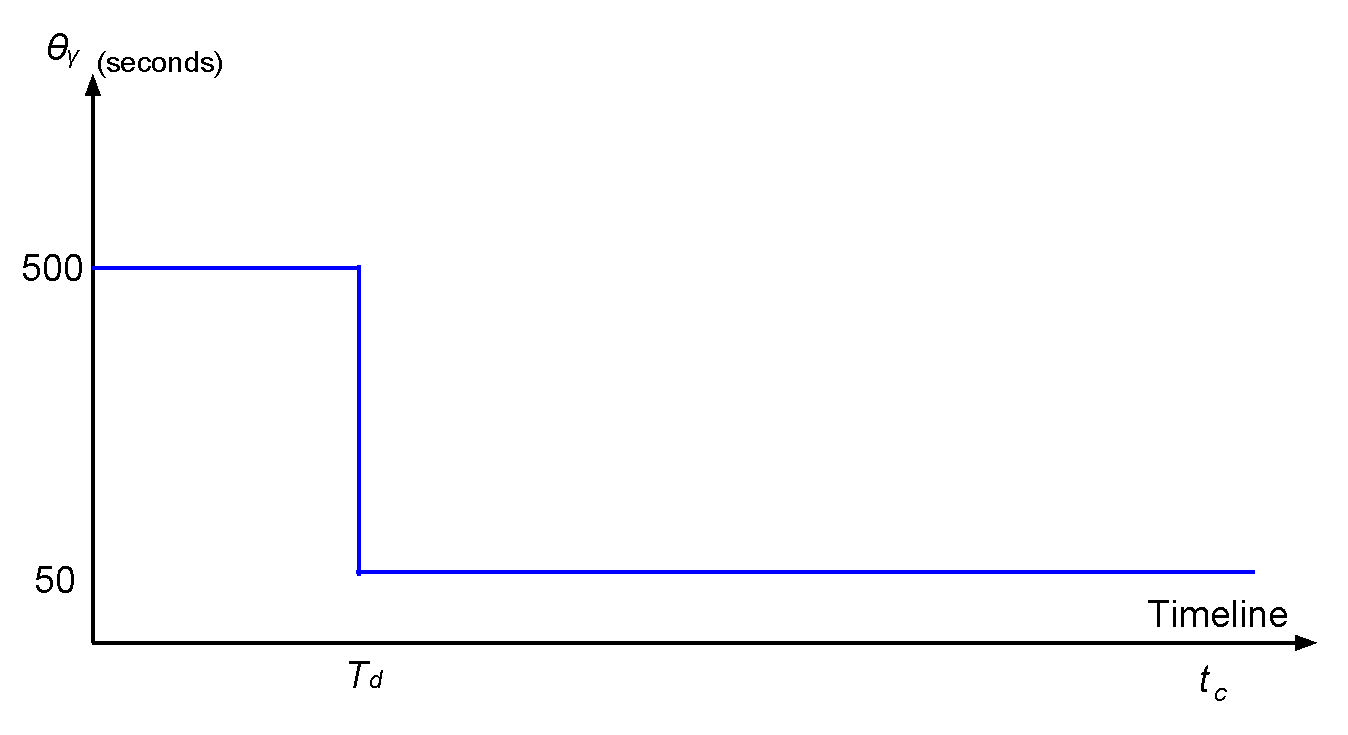
\includegraphics[width=0.6\linewidth]{figures/tolerance/step_signal.pdf} \\
	\caption{A Step Function of $\theta_{\gamma}$. $t_c$ is the current time and $T_d$ is the moment $\theta_{\gamma}$ changes from 500 to 50 seconds}
	\label{fig:evaluation_step_signal}
\end{figure*}

\begin{equation}
\label{eq:step_function}
 \theta_{\gamma}(t_c) =
  \begin{cases}
   50 & \text{if } t_c \geq T_d \\
   500       & \text{if } 0< t_c < T_d
  \end{cases}
\end{equation}

In this experiment, we use two sets of $\theta_{\gamma}$ function. The first one is a step function, in which we decrease $\theta_{\gamma}$ from 500 seconds to 50 seconds at time $T_d$ to simulate the scenario where there are more failures coming than expected. We evaluate the performance difference of dynamic estimation and static estimation while $1000\leq T_d\leq 5000$ based on the estimation of the workflow makespan. The function is shown  in Figure \ref{fig:evaluation_step_signal} and Equation \ref{eq:step_function}, while $t_c$ is the current time. Theoretically speaking, the later we change $\theta_{\gamma}$, the less the reclustering is influenced by the estimation error and thus the less the makespan is. There is one special case when $T_d\to 0$, which means the prior knowledge is wrong at the very beginning. The second one is a pulse wave function, which the amplitude alternates at a steady frequency between fixed minimum (50 seconds) to maximum (500 seconds) values. The function is shown in Figure \ref{fig:evaluation_pulse_signal} and Equation \ref{eq:pulse_function}. $T_c$ is the period and $\tau$ is the duty cycle of the oscillator. It simulates a scenario where the failures follow a periodic pattern \cite{yigitbasi2010analysis} that has been found in many failure traces obtained from production distributed systems. We vary $T_c$ from 1000 seconds to 10000 seconds based on the estimation of workflow makespan and $\tau$ from $0.1T_c$ to $0.5T_c$. 


\begin{figure*}[htb]
	\centering
	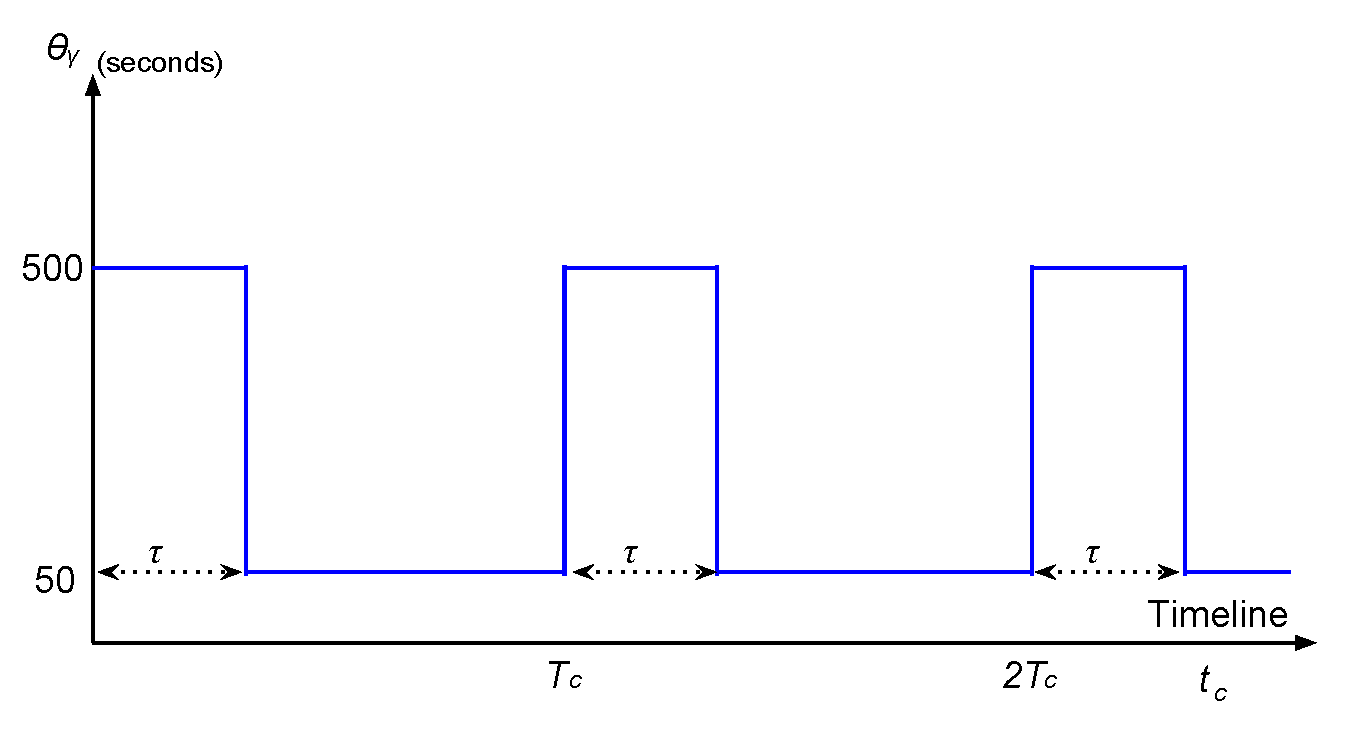
\includegraphics[width=0.6\linewidth]{figures/tolerance/pulse_signal.pdf} \\
	\caption{A Pulse Function of $\theta_{\gamma}$. $t_c$ is the current time and $T_c$ is the period of the wave. $\tau$ is the width of the pulse. }
	\label{fig:evaluation_pulse_signal}
\end{figure*}


\begin{equation}
\label{eq:pulse_function}
 \theta_{\gamma}(t_c) =
  \begin{cases}
   500 & \text{if } 0< t_c \leq \tau \\
   50       & \text{if } \tau< t_c < T_c
  \end{cases}
\end{equation}

Table~\ref{tab:evaluation_methods} summarizes the clustering methods to be evaluated in our experiments. In our experiments, our algorithms take less than 10ms to do the reclustering for each job and thereby they are highly efficient even for large-scale workflows. 
\begin{table*}[!htb]
	%\setlength{\tabcolsep}{11pt}
	\centering
	\small
	\begin{tabular}{l|rrrr}
		\hline
		Abbreviation	& Method	  \\
		\hline
		DR 		& Dynamic Reclustering		\\
		SR 		&Selective Reclustering\\
		VR 	&Vertical Reclustering\\
		HC 	&Horizontal Clustering \\
		\hline
	\end{tabular}
	\caption{Methods to Evaluate in Experiements}
	\label{tab:evaluation_methods}
\end{table*} 


\subsection{Results and discussion}
\label{sec:tolerance:results}

\begin{figure}[!htb]
\centering
  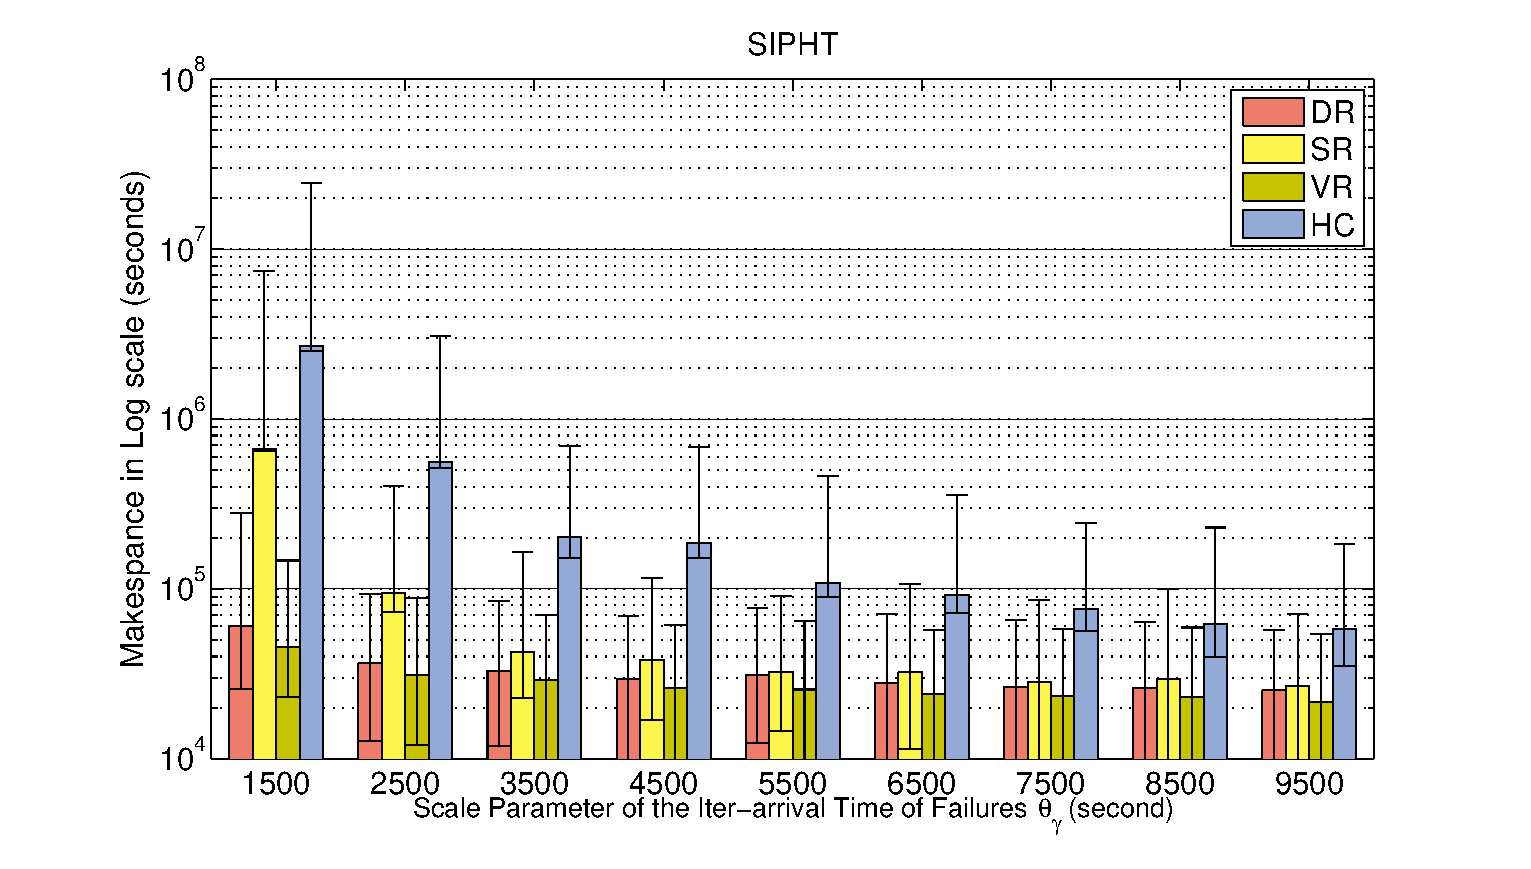
\includegraphics[width=1\linewidth]{figures/tolerance/sipht.eps}
  \caption{Experiment 1: SIPHT Workflow}
  \label{fig:expr_sipht}
\end{figure}

\paragraph{\textbf{Experiment 1}}
Figure~\ref{fig:expr_sipht}, \ref{fig:expr_genome}, \ref{fig:expr_cybershake}, \ref{fig:expr_ligo} and \ref{fig:expr_montage} show the performance of the four reclustering methods (DR, SR, VR and HC) with five workflows respectively. We draw conclusions: 

\begin{figure}[!htb]
\centering
  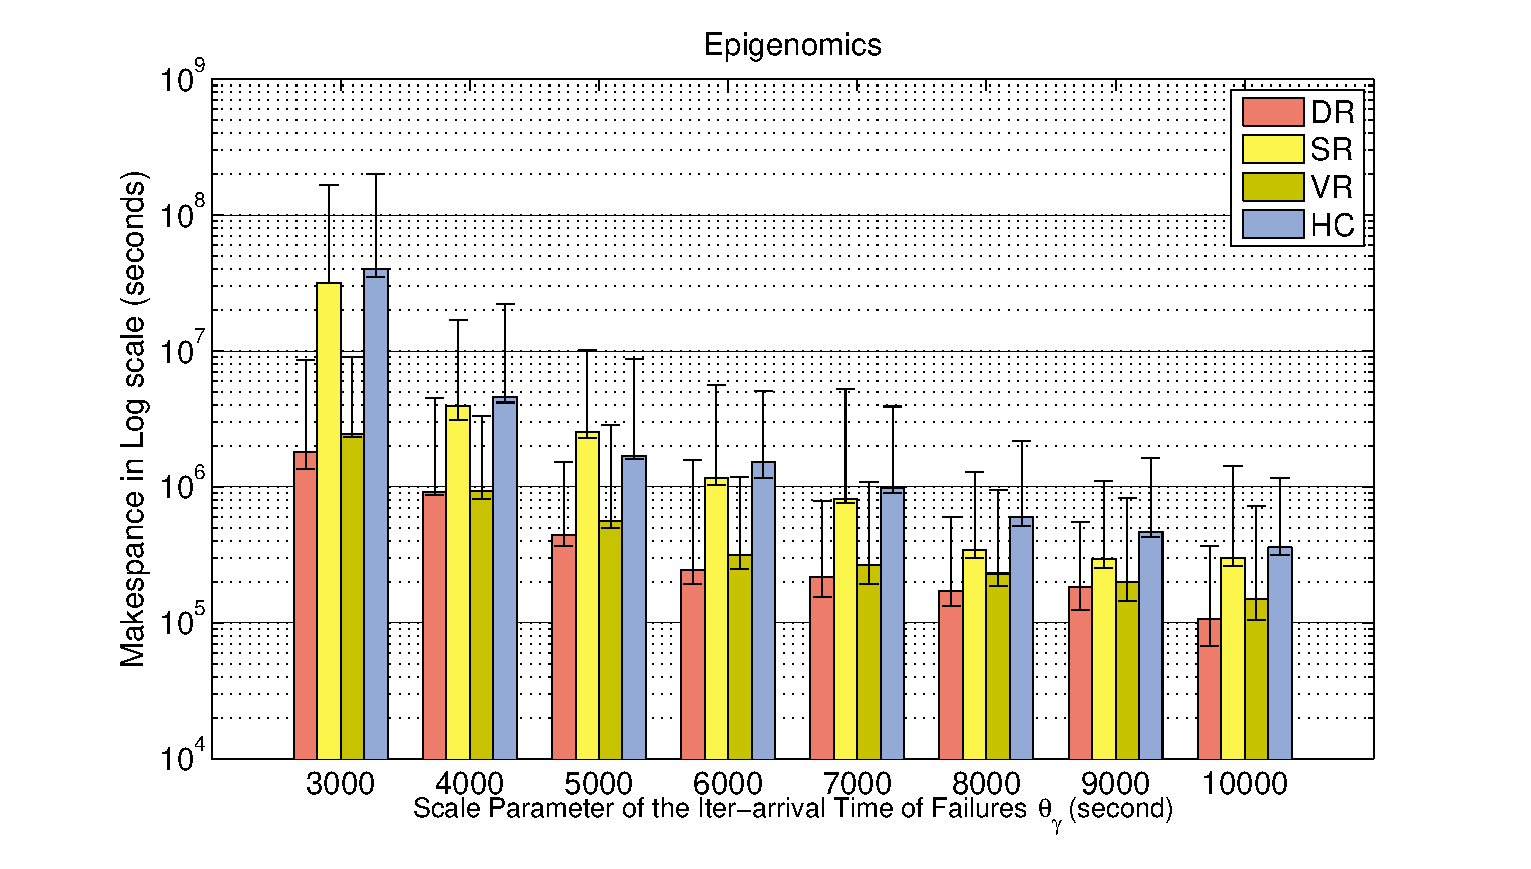
\includegraphics[width=1.0\linewidth]{figures/tolerance/genome.eps}
  \caption{Experiment 1: Epigenomics Workflow}
  \label{fig:expr_genome}
\end{figure}


1). DR, SR and VR have significantly improved the makespan compared to HC in a large scale. By decreasing of the inter-arrival time ($\theta_{\gamma}$) and consequently more failures are generated, the performance difference becomes more significant. 


\begin{figure}[!htb]
\centering
  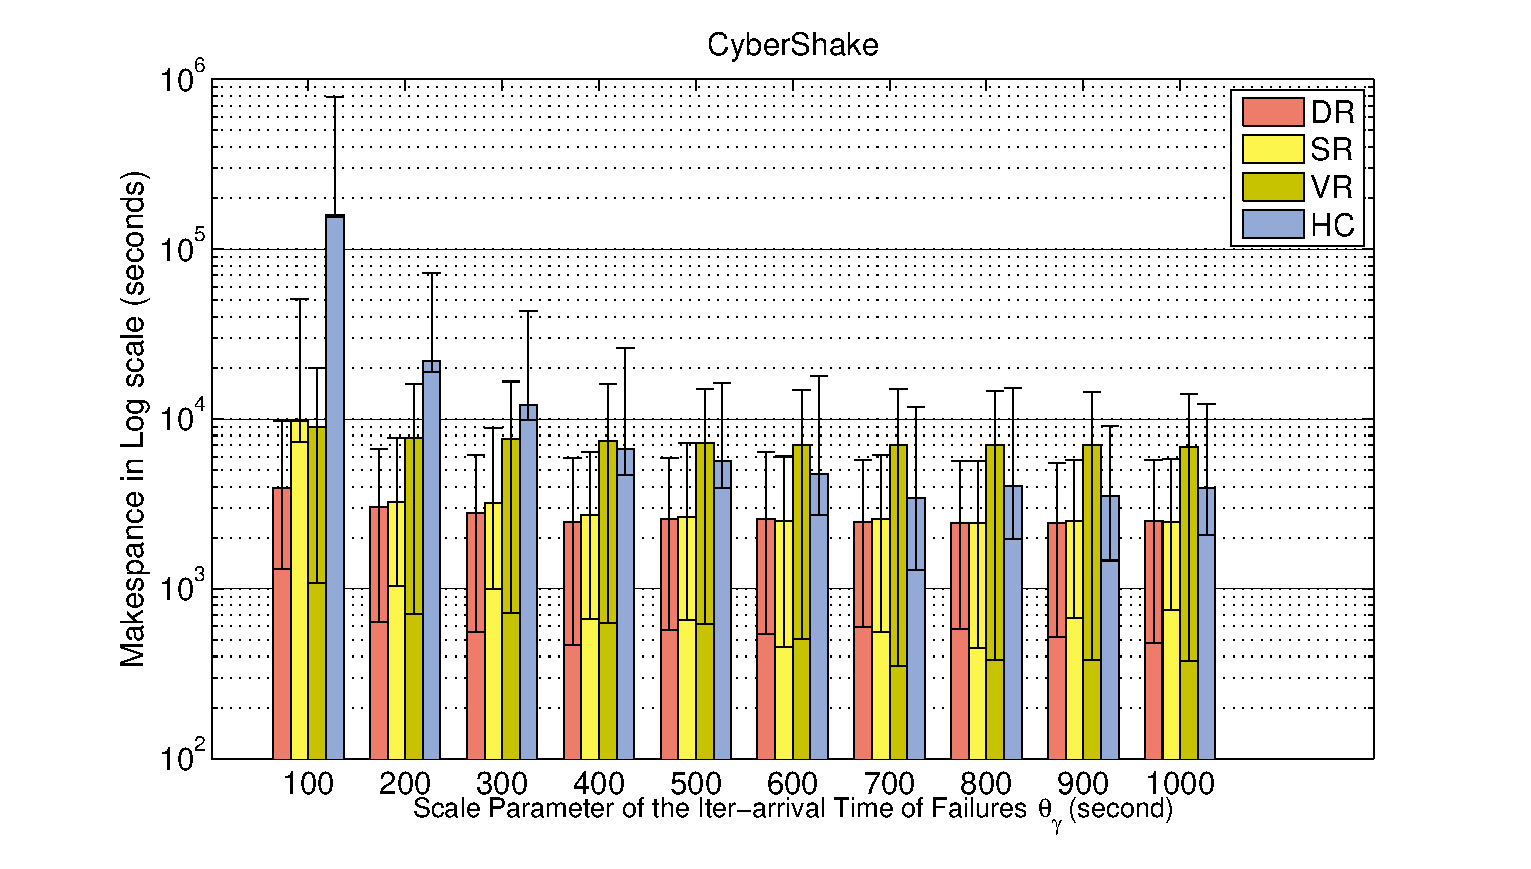
\includegraphics[width=1.0\linewidth]{figures/tolerance/cybershake.eps}
  \caption{Experiment 1: CyberShake Workflow}
  \label{fig:expr_cybershake}
\end{figure}






2). Among the three methods, DR and VR perform consistently better than SR, which fail to improve the makespan when $\theta_{\gamma}$ is small. The reason is the SR does not adjust $k$ according to the occurrence of failures. 
%It is more significant when there is a high failure rate ($\theta_{\gamma}$ is small). 

\begin{figure}[!htb]
\centering
  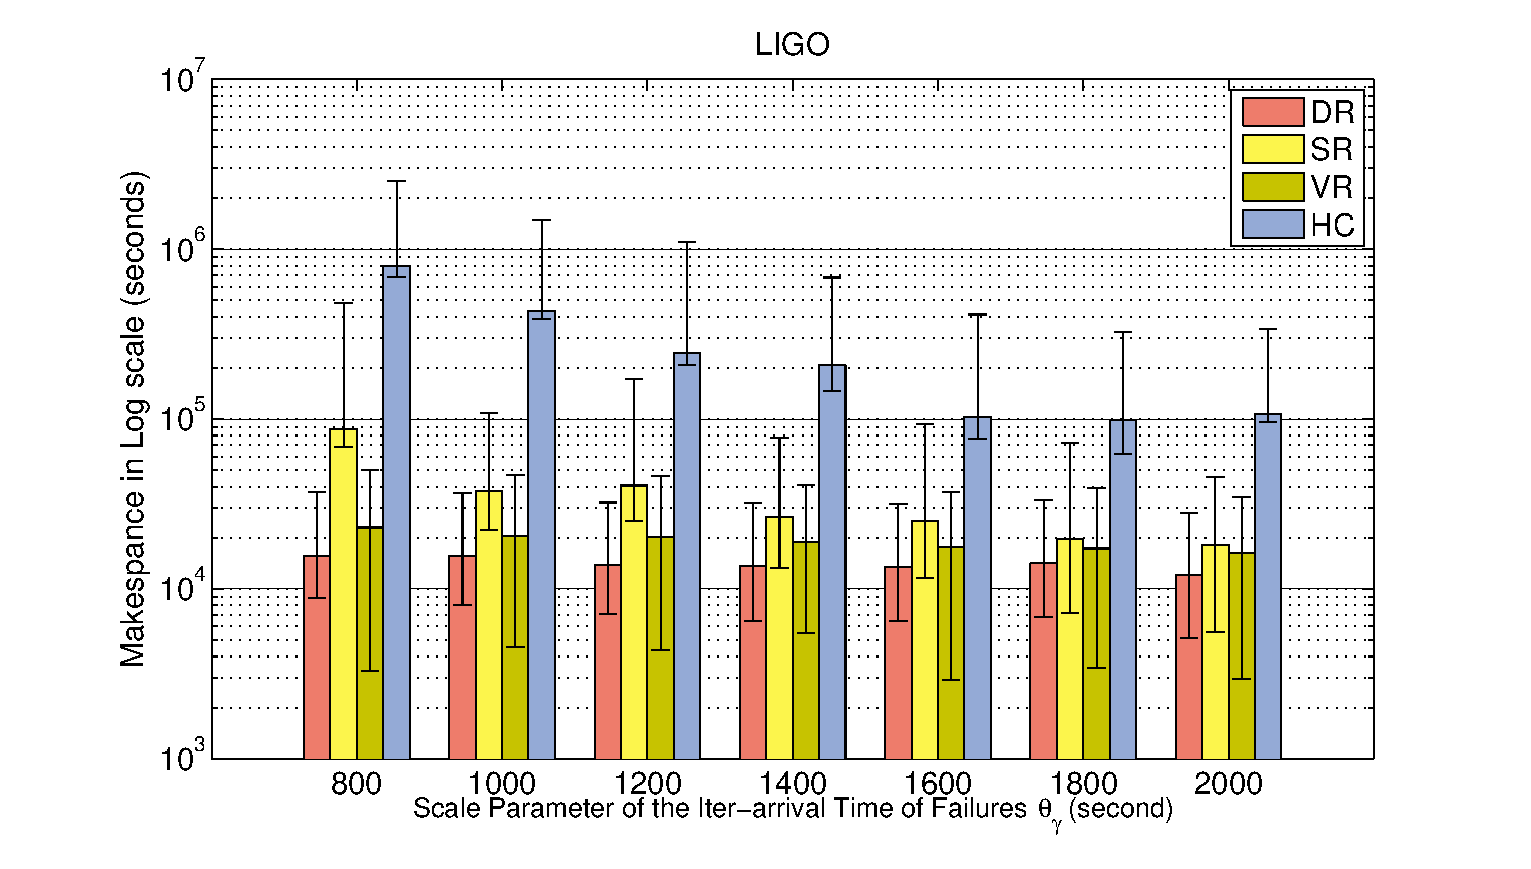
\includegraphics[width=1\linewidth]{figures/tolerance/ligo.eps}
  \caption{Experiment 1: LIGO Workflow}
  \label{fig:expr_ligo}
\end{figure}

3). The performance of VR is highly related to the workflow structure and the average task runtime. For example, according to Figure \ref{fig:model_shape_genome} and Table \ref{tab:model_workflows}, we know that the Epigenomics workflow has a long task runtime (around 50 minutes) and the pipeline length is 4. It means vertical clustering creates really long jobs ($\sim 50\times 4=200$ minutes) and thereby VR is more sensitive to the decrease of $\gamma$. As indicated in Figure \ref{fig:expr_genome}, the makespan increases more significantly with the decrease of $\theta_{\gamma}$ than other workflows. In comparison, the CyberShake workflow does not leave much space for vertical clustering methods to improve since it does not have many pipelines as shown in Figure~\ref{fig:model_shape_cybershake}. In addition, the average task runtime of the CyberShake workflow is relatively short (around 23 seconds). Compared to horizontal methods such as HC, SR and DR, vertical clustering does not generate long jobs and thus the performance of VR is less  sensitive to $\theta_{\gamma}$. 

%4). Under some cases, i.e., the CyberShake workflow, we see that VR does not perform well compared to DR or SR. The reason is the graph structure of the CyberShake workflow does not leave much space for vertical clustering methods to improve since it does not have many pipelines as shown in Figure~\ref{fig:evaluation_shape_cybershake}. DR, a modification of HC, is more likely to improve the performance since most of these workflows have many parallel tasks in the same level. 



\begin{figure}[!htb]
\centering
  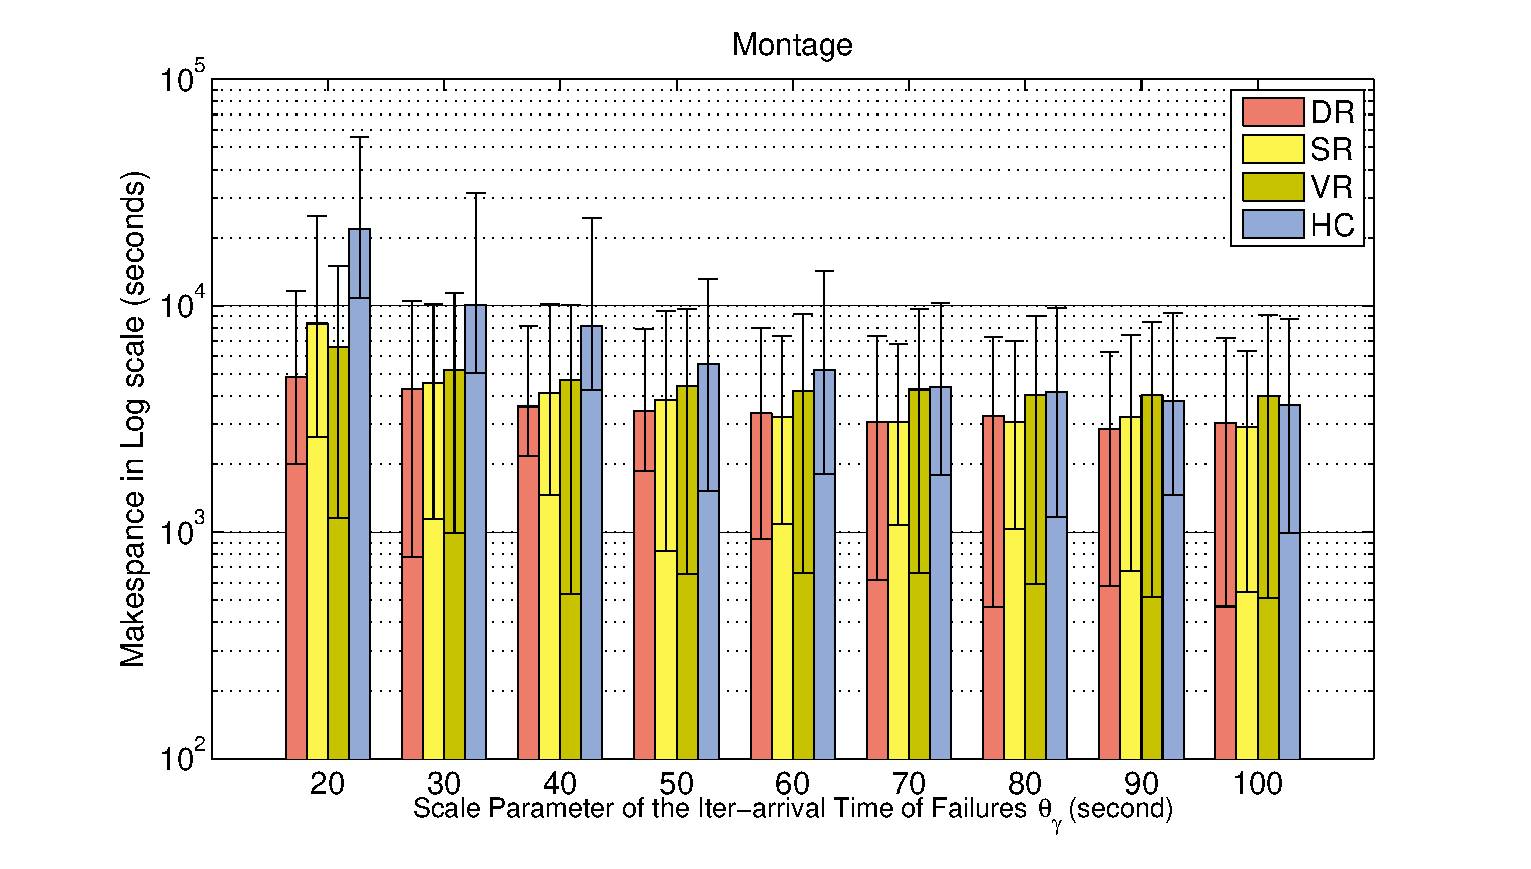
\includegraphics[width=1\linewidth]{figures/tolerance/montage.eps}
  \caption{Experiment 1: Montage Workflow}
  \label{fig:expr_montage}
\end{figure}

\paragraph{\textbf{Experiment 2}}

\begin{figure}[!htb]
\centering
  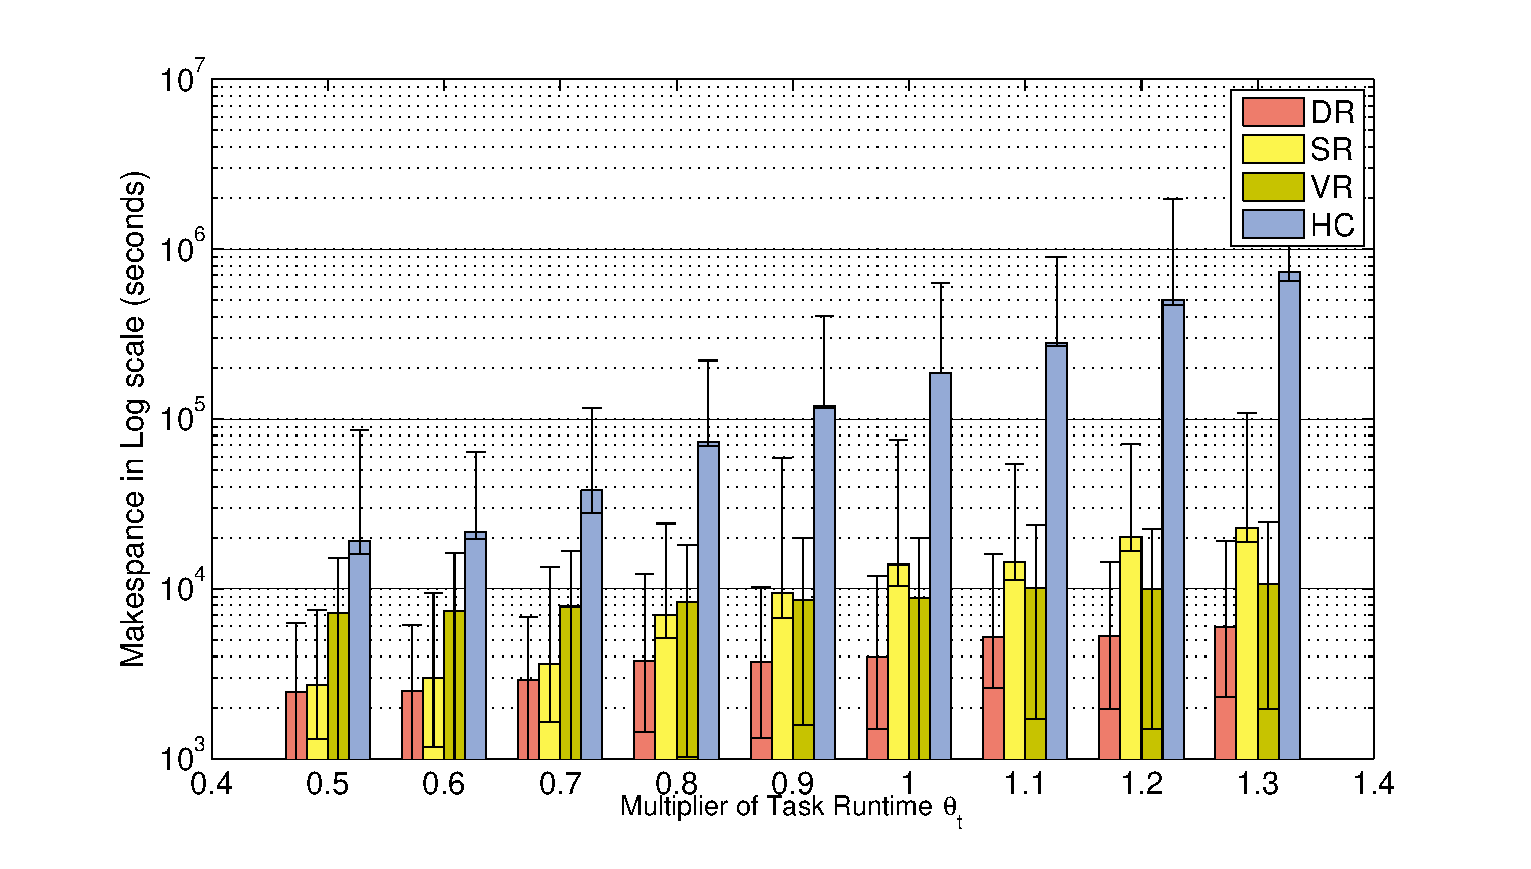
\includegraphics[width=1\linewidth]{figures/tolerance/t.eps}
  \caption{Experiment 2:  Influence of Varying Task Runtime on Makespan (CyberShake)}
  \label{fig:expr_t}
\end{figure}

Figure~\ref{fig:expr_t} shows the performance of our methods with different multiplier of $\theta_{t}$ for the CyberShake workflow. We can see that with the increase of the multiplier, the makespan increases significantly (increase from a scale of $10^4$ to $\sim 10^6$), particularly for HC. The reason is HC is not fault tolerant and it is highly sensitive to the increase of task runtime. While for DR, the reclustering process dynamically adjusts the clustering size based on the estimation of task runtime and thus the performance of DR is more stable. 
%VR?

\begin{figure}[!htb]
\centering
  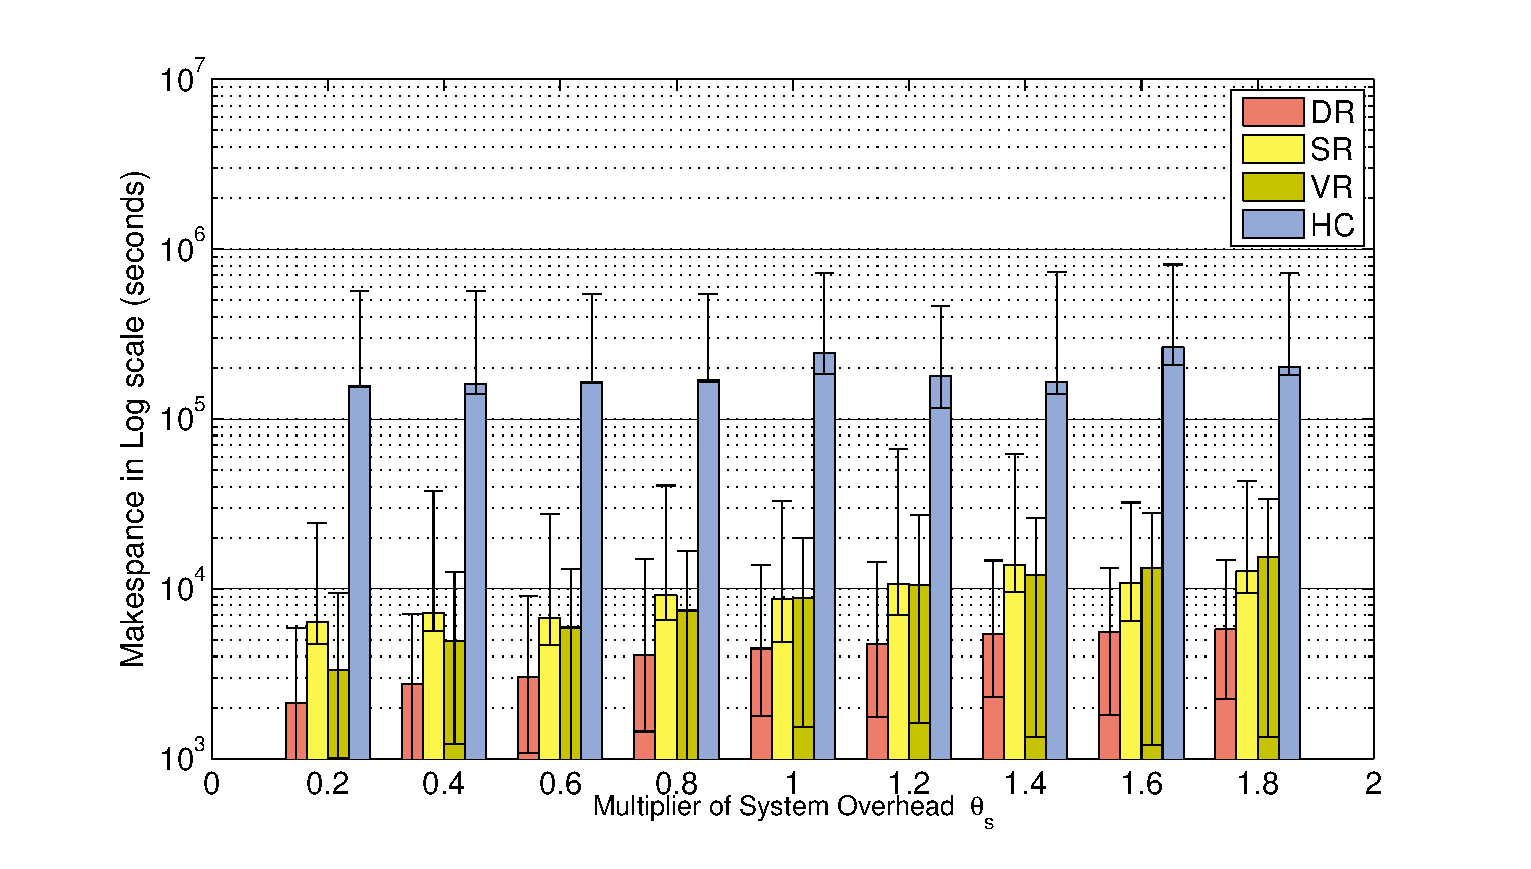
\includegraphics[width=1\linewidth]{figures/tolerance/d.eps}
  \caption{Experiment 2: Influence of Varying System Overhead on Makespan (CyberShake)}
  \label{fig:expr_d}
\end{figure}

Figure~\ref{fig:expr_d} shows the results with different multiplier of $\theta_{s}$ for the CyberShake workflow. Similarly, we can see that with the increase of the multiplier, the makespan increases for all the methods and DR performs best. However, the increase is less significant than that in Figure~\ref{fig:expr_t}. The reason is we may have multiple tasks in a clustered job but only one system overhead per job.


\paragraph{\textbf{Experiment 3}}
\begin{figure}[!htb]
\centering
  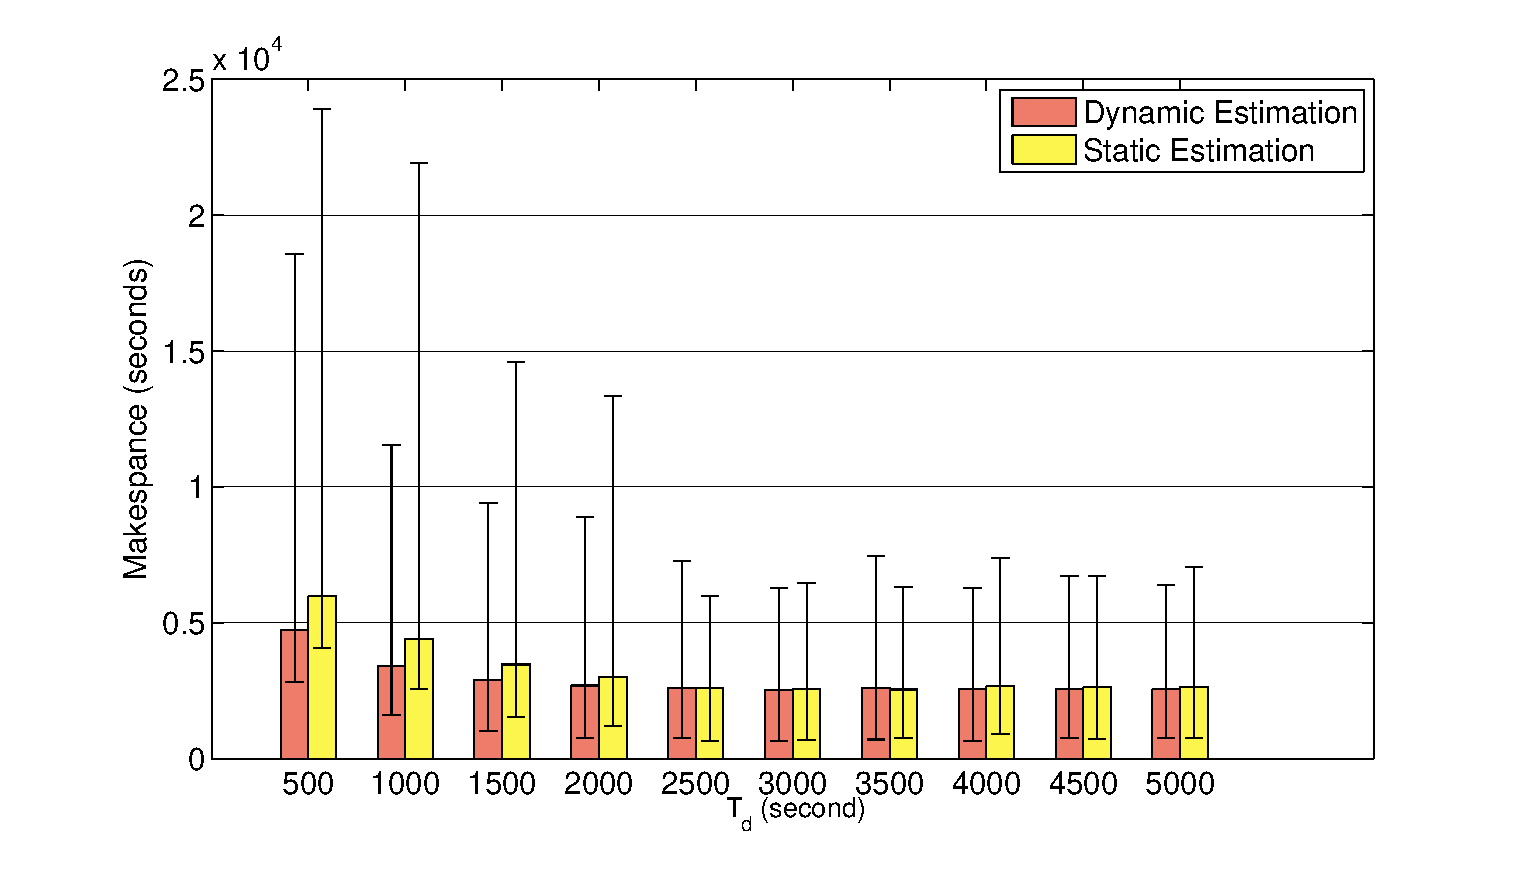
\includegraphics[width=1\linewidth]{figures/tolerance/versus.eps}
  \caption{Experiment 3: Static Estimation vs. Dynamic Estimation (CyberShake, Step Function)}
  \label{fig:expr_static_dynamic}
\end{figure}

Figure~\ref{fig:expr_static_dynamic} further evaluates the performance of the dynamic estimation and static estimation for the CyberShake workflow with a step function of $\theta_{\gamma}$. The reclustering method used in this experiment is DR since it performs best in the last two experiments. In this experiment, we use a step signal and change the inter-arrival time of failures ($\theta_{\gamma}$) from 500 seconds to 50 seconds at $T_d$. We can see that: 1). with the increase of $T_d$, both makespan decrease since the change of  $\theta_{\gamma}$ has less influence on the makespan and there is a lower failure rate on average; 2). Dynamic estimation improves the makespan by up to 22.4\% compared to the static estimation. The reason is the dynamic estimation process is able to update the MLEs of $\theta_{\gamma}$ and decrease the clustering size while the static estimation process does not. 

For the pulse function of $\theta_{\gamma}$, we use $\tau=0.1T_c, 0.3T_c, 0.5T_c$. Figure \ref{fig:expr_pulse_10}, \ref{fig:expr_pulse_30} and \ref{fig:expr_pulse_50} show the performance difference of dynamic estimation and static estimation respectively. When $\tau=0.1T_c$, DR with dynamic estimation improves the makespan by up to 25.7\% compared to case with static estimation. When $\tau=0.3T_c$, the performance difference between dynamic estimation and static estimation is up to 27.3\%. We can also see that when $T_c$ is small (i.e., $T_c=1000$), the performance difference is not significant since the inter-arrival time of failures changes frequently and the dynamic estimation process is not able to update swiftly. While when $T_c$ is 10000, the performance difference is not significant neither since the period is too long and the workflow has completed successfully. When $\tau=0.5T_c$, the performance different between dynamic estimation and static estimation is up to 9.1\%, since the high $\theta_{\gamma}$ and the low $\theta_{\gamma}$ have equal influence on the failure occurrence. 


\begin{figure}[!htb]
\centering
  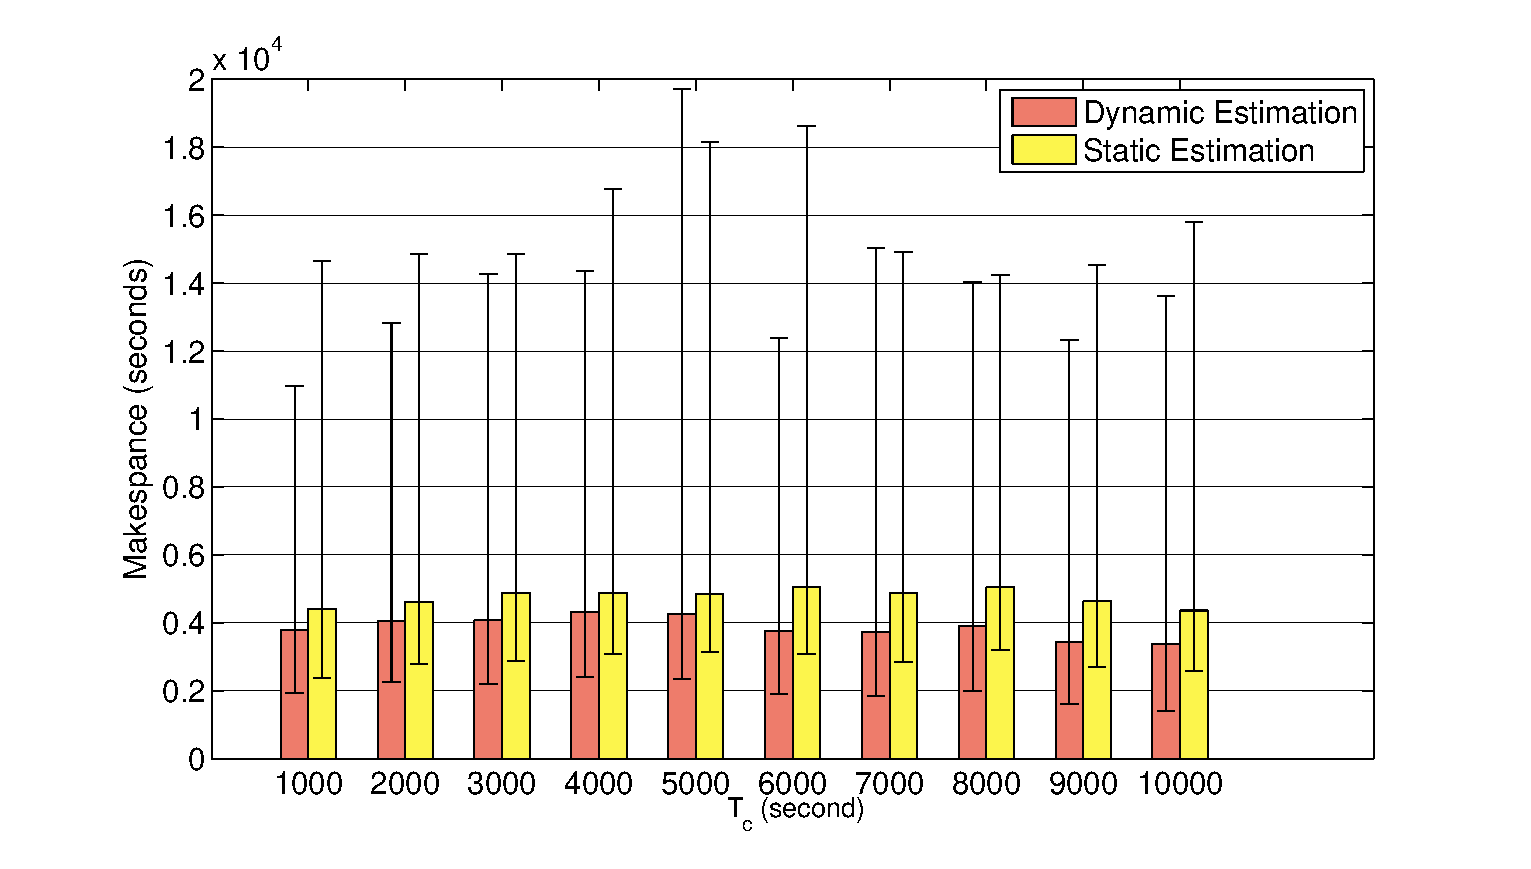
\includegraphics[width=1\linewidth]{figures/tolerance/pulse_t10.eps}
  \caption{Experiment 3: Static Estimation vs. Dynamic Estimation (CyberShake, Pulse Function ($\tau=0.1T_c$))}
  \label{fig:expr_pulse_10}
\end{figure}

\begin{figure}[!htb]
\centering
  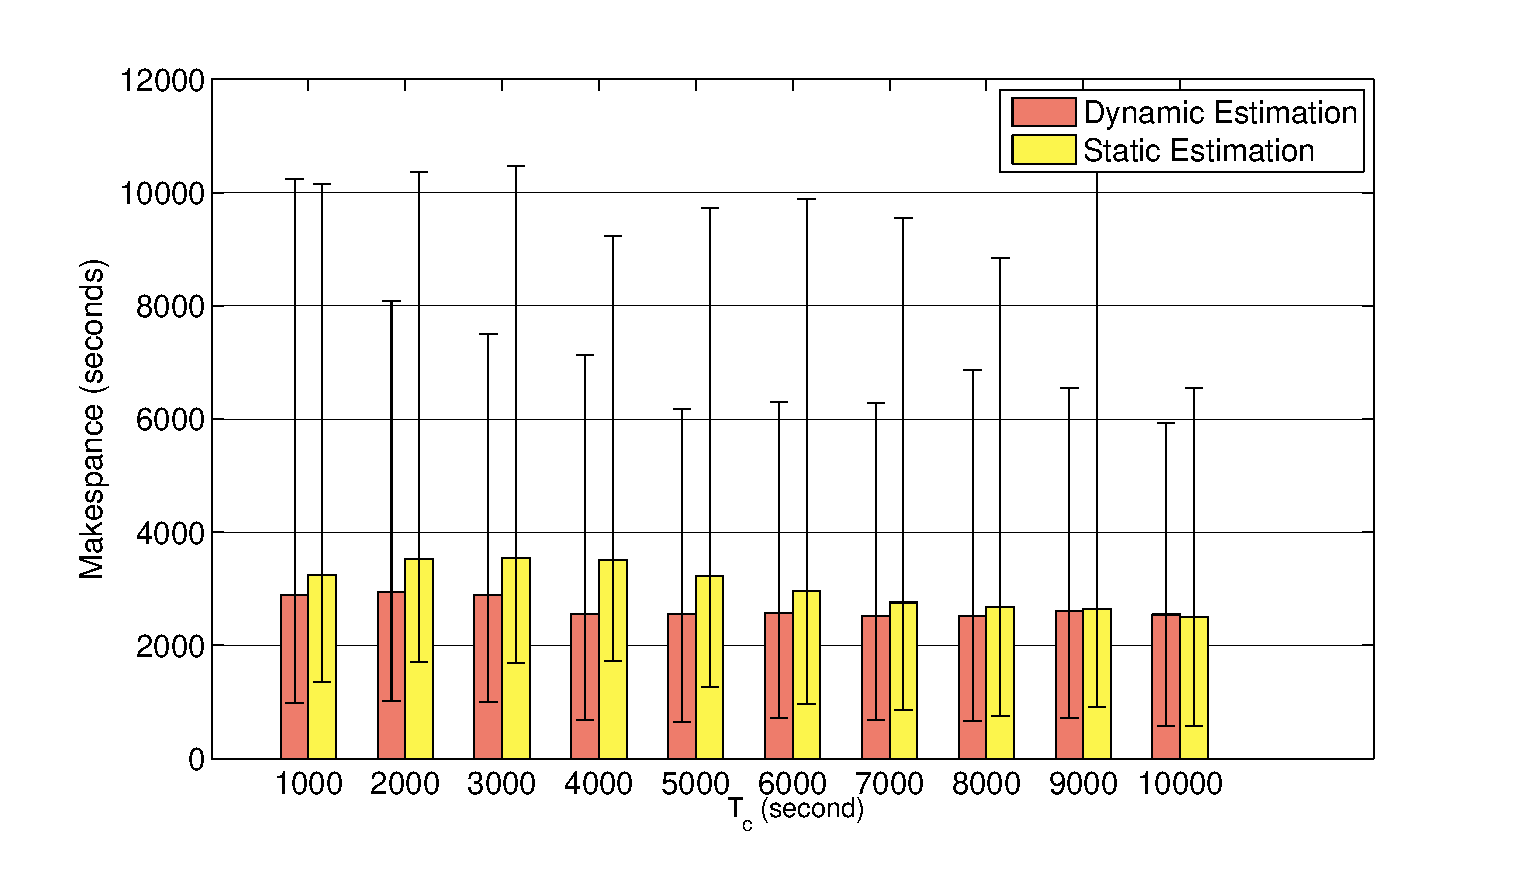
\includegraphics[width=1\linewidth]{figures/tolerance/pulse_t30.eps}
  \caption{Experiment 3: Static Estimation vs. Dynamic Estimation (CyberShake, Pulse Function ($\tau=0.3T_c$))}
  \label{fig:expr_pulse_30}
\end{figure}

\begin{figure}[!htb]
\centering
  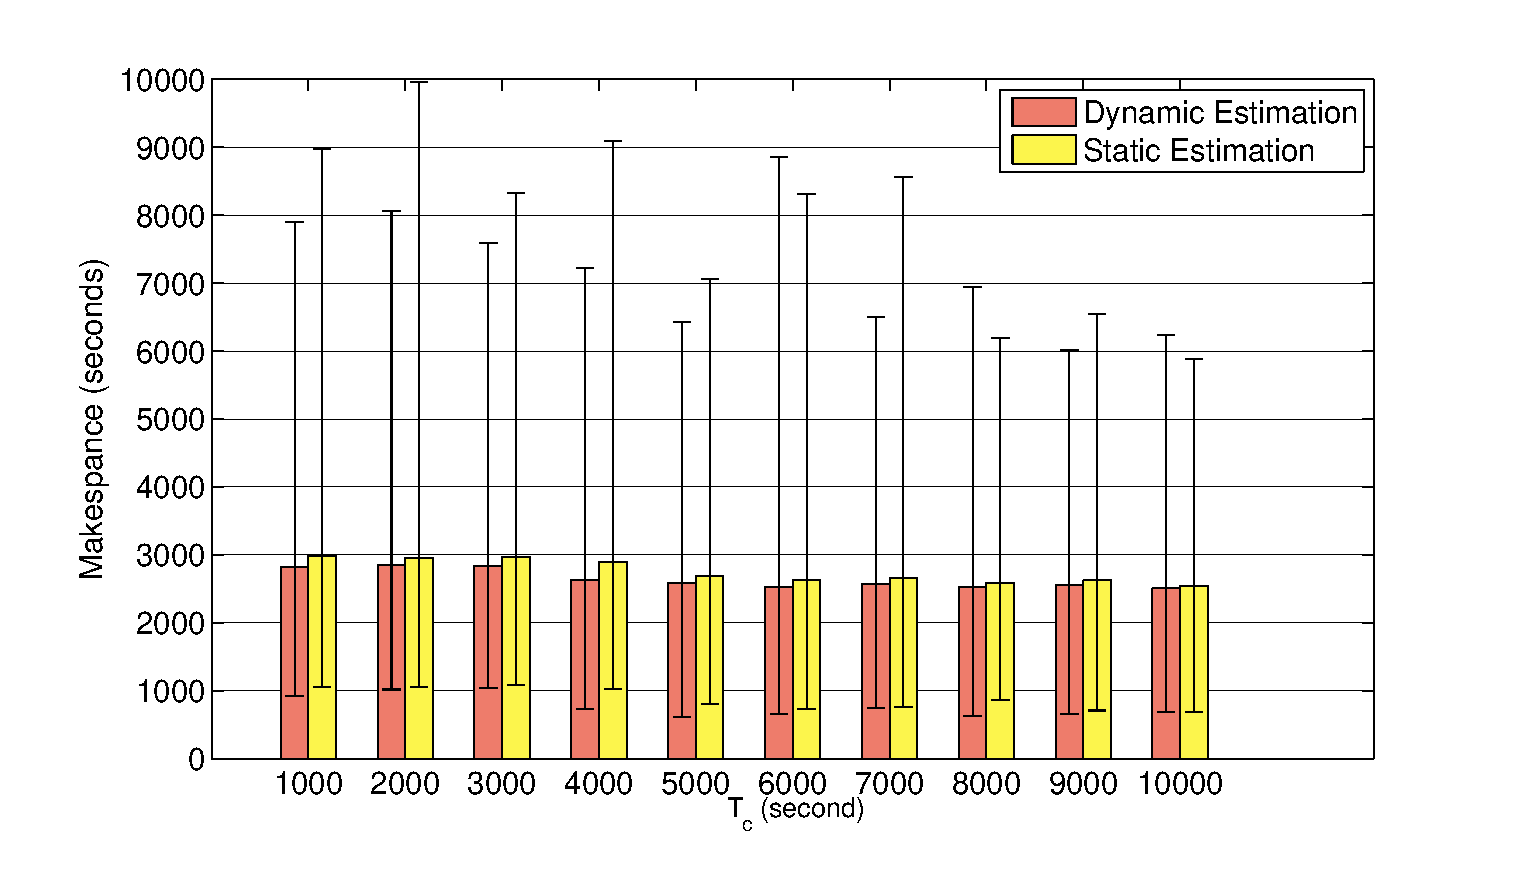
\includegraphics[width=1\linewidth]{figures/tolerance/pulse_t50.eps}
  \caption{Experiment 3: Static Estimation vs. Dynamic Estimation (CyberShake, Pulse Function ($\tau=0.5T_c$))}
  \label{fig:expr_pulse_50}
\end{figure}


\section{Summary}
In this chapter, we model transient failures in a distributed environment and assess their influence of task clustering. We propose three dynamic clustering methods to improve the fault tolerance of task clustering and apply them to five widely used scientific workflows. From our experiments, we conclude that the three proposed methods improve the makespan significantly compared to an existing algorithm widely used in workflow management systems. In particular, our Dynamic Reclustering method performs best among the three methods since it can adjust the clustering size based on the Maximum Likelihood Estimation of task runtime, system overheads and the inter-arrival time of failures. Our Vertical Reclustering method improves the performance significantly for  workflows that have a short task runtime. Our dynamic estimation using on-going data collected from the workflow execution can further improve the fault tolerance in a dynamic environment where the inter-arrival time of failures is fluctuant. 
